
\documentclass{article}\usepackage[]{graphicx}\usepackage[]{color}
%% maxwidth is the original width if it is less than linewidth
%% otherwise use linewidth (to make sure the graphics do not exceed the margin)
\makeatletter
\def\maxwidth{ %
  \ifdim\Gin@nat@width>\linewidth
    \linewidth
  \else
    \Gin@nat@width
  \fi
}
\makeatother

\definecolor{fgcolor}{rgb}{0.345, 0.345, 0.345}
\newcommand{\hlnum}[1]{\textcolor[rgb]{0.686,0.059,0.569}{#1}}%
\newcommand{\hlstr}[1]{\textcolor[rgb]{0.192,0.494,0.8}{#1}}%
\newcommand{\hlcom}[1]{\textcolor[rgb]{0.678,0.584,0.686}{\textit{#1}}}%
\newcommand{\hlopt}[1]{\textcolor[rgb]{0,0,0}{#1}}%
\newcommand{\hlstd}[1]{\textcolor[rgb]{0.345,0.345,0.345}{#1}}%
\newcommand{\hlkwa}[1]{\textcolor[rgb]{0.161,0.373,0.58}{\textbf{#1}}}%
\newcommand{\hlkwb}[1]{\textcolor[rgb]{0.69,0.353,0.396}{#1}}%
\newcommand{\hlkwc}[1]{\textcolor[rgb]{0.333,0.667,0.333}{#1}}%
\newcommand{\hlkwd}[1]{\textcolor[rgb]{0.737,0.353,0.396}{\textbf{#1}}}%
\let\hlipl\hlkwb

\usepackage{framed}
\makeatletter
\newenvironment{kframe}{%
 \def\at@end@of@kframe{}%
 \ifinner\ifhmode%
  \def\at@end@of@kframe{\end{minipage}}%
  \begin{minipage}{\columnwidth}%
 \fi\fi%
 \def\FrameCommand##1{\hskip\@totalleftmargin \hskip-\fboxsep
 \colorbox{shadecolor}{##1}\hskip-\fboxsep
     % There is no \\@totalrightmargin, so:
     \hskip-\linewidth \hskip-\@totalleftmargin \hskip\columnwidth}%
 \MakeFramed {\advance\hsize-\width
   \@totalleftmargin\z@ \linewidth\hsize
   \@setminipage}}%
 {\par\unskip\endMakeFramed%
 \at@end@of@kframe}
\makeatother

\definecolor{shadecolor}{rgb}{.97, .97, .97}
\definecolor{messagecolor}{rgb}{0, 0, 0}
\definecolor{warningcolor}{rgb}{1, 0, 1}
\definecolor{errorcolor}{rgb}{1, 0, 0}
\newenvironment{knitrout}{}{} % an empty environment to be redefined in TeX

\usepackage{alltt}

\usepackage{fancyhdr} % Required for custom headers
\usepackage{lastpage} % Required to determine the last page for the footer
\usepackage{extramarks} % Required for headers and footers
%\usepackage[usenames,dvipsnames]{color} % Required for custom colors
\usepackage{graphicx} % Required to insert images
\usepackage{listings} % Required for insertion of code
\usepackage{courier} % Required for the courier font
\usepackage[utf8]{inputenc}
\usepackage[english]{babel}
\usepackage{amsmath,amsfonts,amsthm,bbm} 
\usepackage{float}
\usepackage{hyperref}

% Margins
\topmargin=-0.45in
\evensidemargin=0in
\oddsidemargin=0in
\textwidth=6.5in
\textheight=9.0in
\headsep=0.25in

\linespread{1.1} % Line spacing

% Set up the header and footer
\pagestyle{fancy}
\lhead{\hmwkAuthorName} % Top left header
\chead{\hmwkClass\ (\hmwkClassInstructor\ \hmwkClassTime): \hmwkTitle} % Top center head
\rhead{\firstxmark} % Top right header
\lfoot{\lastxmark} % Bottom left footer
\cfoot{} % Bottom center footer
\rfoot{Page\ \thepage\ of\ \protect\pageref{LastPage}} % Bottom right footer
\renewcommand\headrulewidth{0.4pt} % Size of the header rule
\renewcommand\footrulewidth{0.4pt} % Size of the footer rule

\setlength\parindent{0pt} % Removes all indentation from paragraphs


%----------------------------------------------------------------------------------------
%	DOCUMENT STRUCTURE COMMANDS
%	Skip this unless you know what you're doing
%----------------------------------------------------------------------------------------

% Header and footer for when a page split occurs within a problem environment
\newcommand{\enterProblemHeader}[1]{
\nobreak\extramarks{#1}{#1 continued on next page\ldots}\nobreak
\nobreak\extramarks{#1 (continued)}{#1 continued on next page\ldots}\nobreak
}

% Header and footer for when a page split occurs between problem environments
\newcommand{\exitProblemHeader}[1]{
\nobreak\extramarks{#1 (continued)}{#1 continued on next page\ldots}\nobreak
\nobreak\extramarks{#1}{}\nobreak
}

\setcounter{secnumdepth}{0} % Removes default section numbers
\newcounter{homeworkProblemCounter} % Creates a counter to keep track of the number of problems

\newcommand{\homeworkProblemName}{}
\newenvironment{homeworkProblem}[1][Problem \arabic{homeworkProblemCounter}]{ % Makes a new environment called homeworkProblem which takes 1 argument (custom name) but the default is "Problem #"
\stepcounter{homeworkProblemCounter} % Increase counter for number of problems
\renewcommand{\homeworkProblemName}{#1} % Assign \homeworkProblemName the name of the problem
\section{\homeworkProblemName} % Make a section in the document with the custom problem count
\enterProblemHeader{\homeworkProblemName} % Header and footer within the environment
}{
\exitProblemHeader{\homeworkProblemName} % Header and footer after the environment
}

\newcommand{\problemAnswer}[1]{ % Defines the problem answer command with the content as the only argument
\noindent\framebox[\columnwidth][c]{\begin{minipage}{0.98\columnwidth}#1\end{minipage}} % Makes the box around the problem answer and puts the content inside
}

\newcommand{\homeworkSectionName}{}
\newenvironment{homeworkSection}[1]{ % New environment for sections within homework problems, takes 1 argument - the name of the section
\renewcommand{\homeworkSectionName}{#1} % Assign \homeworkSectionName to the name of the section from the environment argument
\subsection{\homeworkSectionName} % Make a subsection with the custom name of the subsection
\enterProblemHeader{\homeworkProblemName\ [\homeworkSectionName]} % Header and footer within the environment
}{
\enterProblemHeader{\homeworkProblemName} % Header and footer after the environment
}

%----------------------------------------------------------------------------------------
%	NAME AND CLASS SECTION
%----------------------------------------------------------------------------------------

\newcommand{\hmwkTitle}{MCMC} % Assignment title
\newcommand{\hmwkDueDate}{1} % Due date
\newcommand{\hmwkClass}{MCMC} % Course/class
\newcommand{\hmwkClassTime}{} % Class/lecture time
\newcommand{\hmwkClassInstructor}{Prof.} % Teacher/lecturer
\newcommand{\hmwkAuthorName}{Peiliang Guo} % Your name

%----------------------------------------------------------------------------------------
%	TITLE PAGE
%----------------------------------------------------------------------------------------

\title{
\vspace{2in}
\textmd{\textbf{\hmwkClass:\ \hmwkTitle}}\\
\normalsize\vspace{0.1in}\small{Due\ on\ \hmwkDueDate}\\
\vspace{0.1in}\large{\textit{\hmwkClassInstructor\ \hmwkClassTime}}
\vspace{3in}
}

\author{\textbf{\hmwkAuthorName}}
\date{} % Insert date here if you want it to appear below your name

%----------------------------------------------------------------------------------------
\IfFileExists{upquote.sty}{\usepackage{upquote}}{}
\begin{document}


\newpage

\begin{homeworkProblem}

Write and run a computer program to compute a Monte Carlo (including standard errors) of $\mathbb{E}((Y+Z)/(1+|Z|))$, where $Y~$ Exponential(3) and $Z~$ Normal(0,1) are independent.\\
Source code:\\
\begin{knitrout}
\definecolor{shadecolor}{rgb}{0.969, 0.969, 0.969}\color{fgcolor}\begin{kframe}
\begin{alltt}
\hlcom{#Estimate E((Y+Z)/(1+|Z|)) where Y~Exp(3) and Z~normal(0,1) and are independent}
\hlstd{fn} \hlkwb{=} \hlkwa{function}\hlstd{(}\hlkwc{y}\hlstd{,}\hlkwc{z}\hlstd{) \{(y}\hlopt{+}\hlstd{z)}\hlopt{/}\hlstd{(}\hlnum{1}\hlopt{+}\hlkwd{abs}\hlstd{(z))\}}

\hlcom{#number of cases}
\hlstd{M}\hlkwb{=}\hlnum{10}\hlopt{^}\hlnum{6}

\hlstd{ylist} \hlkwb{=} \hlkwd{rexp}\hlstd{(M,}\hlnum{3}\hlstd{)}
\hlstd{zlist} \hlkwb{=} \hlkwd{rnorm}\hlstd{(M)}
\hlstd{funclist} \hlkwb{=} \hlkwd{fn}\hlstd{(ylist,zlist)}
\hlstd{funcmean} \hlkwb{=} \hlkwd{mean}\hlstd{(funclist)}
\hlstd{funcse} \hlkwb{=} \hlkwd{sd}\hlstd{(funclist)}\hlopt{/}\hlkwd{sqrt}\hlstd{(M)}
\hlkwd{cat}\hlstd{(}\hlstr{'Estimate E((Y+Z)/(1+|Z|)) where Y~Exp(3) and Z~Normal(0,1)\textbackslash{}n'}\hlstd{)}
\hlkwd{cat}\hlstd{(}\hlstr{'M = '}\hlstd{,M,}\hlstr{'\textbackslash{}n'}\hlstd{)}
\hlkwd{cat}\hlstd{(}\hlstr{'estimate = '}\hlstd{,funcmean,}\hlstr{'\textbackslash{}n'}\hlstd{)}
\hlkwd{cat}\hlstd{(}\hlstr{'standard error = '}\hlstd{,funcse,}\hlstr{'\textbackslash{}n'}\hlstd{)}
\end{alltt}
\end{kframe}
\end{knitrout}
Output of several runs:
\begin{knitrout}
\definecolor{shadecolor}{rgb}{0.969, 0.969, 0.969}\color{fgcolor}\begin{kframe}
\begin{verbatim}
## Estimate E((Y+Z)/(1+|Z|)) where Y~Exp(3) and Z~Normal(0,1)
## M =  1e+06 
## estimate =  0.2054176 
## standard error =  0.0004825309
## Estimate E((Y+Z)/(1+|Z|)) where Y~Exp(3) and Z~Normal(0,1)
## M =  1e+06 
## estimate =  0.2056342 
## standard error =  0.0004829007
## Estimate E((Y+Z)/(1+|Z|)) where Y~Exp(3) and Z~Normal(0,1)
## M =  1e+06 
## estimate =  0.2047581 
## standard error =  0.0004828433
## Estimate E((Y+Z)/(1+|Z|)) where Y~Exp(3) and Z~Normal(0,1)
## M =  1e+06 
## estimate =  0.2045917 
## standard error =  0.0004823873
## Estimate E((Y+Z)/(1+|Z|)) where Y~Exp(3) and Z~Normal(0,1)
## M =  1e+06 
## estimate =  0.2043318 
## standard error =  0.0004820518
\end{verbatim}
\end{kframe}
\end{knitrout}
The tabulated result is as follows:\\
\center
\begin{knitrout}
\definecolor{shadecolor}{rgb}{0.969, 0.969, 0.969}\color{fgcolor}
\begin{tabular}{r|r}
\hline
estimation & standard\_error\\
\hline
0.2054176 & 0.0004825\\
\hline
0.2056342 & 0.0004829\\
\hline
0.2047581 & 0.0004828\\
\hline
0.2045917 & 0.0004824\\
\hline
0.2043318 & 0.0004821\\
\hline
\end{tabular}


\end{knitrout}
The estimated value for $\mathbb{E}((Y+Z)/(1+|Z|))$ is 0.205 with standard error of approximately \ensuremath{4.8\times 10^{-4}}. The results from the five runs are quite consistent. The number of samples taken for the estimation is set to be $10^6$, as this number gives consistent results with reasonable computation power (runs within 1 second). 

\end{homeworkProblem}

\begin{homeworkProblem}

Re-write the integral
$$I:=\int_1^\infty\left(\int_{-\infty}^\infty(1+x^2+\sin(x))^{-|y|^3-2}\,dy \right)\,dx$$
as some expected value, and then estimate $I$ using Monte Carlo algorithm.\\
\\
The interval of integration of $x$ is from $1$ to $\infty$, so we choose $x$ to follow a shifted exponential distribution, i.e. $x-1$ follows a exponential($\lambda$) distribution, and the value of $\lambda$ is set to $1$, by trial and error to minimize standard error. The interval of integration of $y$ is $-\infty$ to $\infty$, so we can choose $y$ to follow a Normal$(0,\sigma^2)$ distribution, and the value $\sigma$ is also found to be 1 by methods of trial and error. 
Now, we can write the integral as
\begin{align*}
I:&=\int_1^\infty\left(\int_{-\infty}^\infty(1+x^2+\sin(x))^{-|y|^3-2}\,dy \right)\,dx\\
  &=\int_1^\infty\int_{-\infty}^\infty(1+x^2+\sin(x))^{-|y|^3-2}\sqrt{2\pi}e^{\frac{y^2}{2}}\,\left(\frac{1}{\sqrt{2\pi}}e^{-\frac{y^2}{2}}dy\right) \,dx\\
  &=\int_1^\infty\int_{-\infty}^\infty(1+x^2+\sin(x))^{-|y|^3-2}\sqrt{2\pi}e^{\frac{y^2}{2}}\frac{1}{}e^{(x-1)}\,\left(\frac{1}{\sqrt{2\pi}}e^{-\frac{y^2}{2}}dy\right) \,\left( e^{-(x-1)}dx\right)\\
  &=\int_0^\infty\int_{-\infty}^\infty(1+(x+1)^2+\sin(x+1))^{-|y|^3-2}\sqrt{2\pi}e^{\frac{y^2}{2}}\frac{1}{}e^{ x}\,\left(\frac{1}{\sqrt{2\pi}}e^{-\frac{y^2}{2}}dy\right) \,\left( e^{- x}dx\right)\\
  &=\mathbb{E}\left[{\sqrt{2\pi}}(X^2+2X+2+\sin(X+1))^{-|Y|^3-2}\exp\{\frac{Y^2}{2}+X\}\right],
\end{align*}
where $X$ follows a Exponential($1$) distribution and $Y$ follows a Normal($0,1$) distribution.

Source code:\\
\begin{knitrout}
\definecolor{shadecolor}{rgb}{0.969, 0.969, 0.969}\color{fgcolor}\begin{kframe}
\begin{alltt}
\hlcom{#Estimate E[(sigma(2pi)^0.5\textbackslash{}lambda)(X^2+2X+2+sin(X+1))^(-|Y|^3-2)exp(Y^2/2sigma^2+X)]}
\hlcom{#where X~Exp(lambda) and Y~normal(0,sigma^2) and are independent}
\hlstd{sigma} \hlkwb{=} \hlnum{1}
\hlstd{lambda} \hlkwb{=} \hlnum{1}
\hlstd{fn} \hlkwb{=} \hlkwa{function}\hlstd{(}\hlkwc{x}\hlstd{,}\hlkwc{y}\hlstd{)}
  \hlstd{\{sigma}\hlopt{/}\hlstd{lambda}\hlopt{*}\hlkwd{sqrt}\hlstd{(}\hlnum{2}\hlopt{*}\hlstd{pi)}\hlopt{*}\hlstd{(x}\hlopt{^}\hlnum{2}\hlopt{+}\hlnum{2}\hlopt{*}\hlstd{x}\hlopt{+}\hlnum{2}\hlopt{+}\hlkwd{sin}\hlstd{(x}\hlopt{+}\hlnum{1}\hlstd{))}\hlopt{^}\hlstd{(}\hlopt{-}\hlnum{2}\hlopt{-}\hlstd{(}\hlkwd{abs}\hlstd{(y))}\hlopt{^}\hlnum{3}\hlstd{)}\hlopt{*}\hlkwd{exp}\hlstd{(y}\hlopt{^}\hlnum{2}\hlopt{/}\hlnum{2}\hlopt{/}\hlstd{sigma}\hlopt{^}\hlnum{2}\hlopt{+}\hlstd{x)\}}

\hlcom{#number of cases}
\hlstd{M}\hlkwb{=}\hlnum{10}\hlopt{^}\hlnum{6}

\hlstd{xlist} \hlkwb{=} \hlkwd{rexp}\hlstd{(M,}\hlnum{1}\hlopt{/}\hlstd{lambda)}
\hlstd{ylist} \hlkwb{=} \hlkwd{rnorm}\hlstd{(M,}\hlnum{0}\hlstd{,sigma)}
\hlstd{funclist} \hlkwb{=} \hlkwd{fn}\hlstd{(xlist,ylist)}
\hlstd{funcmean} \hlkwb{=} \hlkwd{mean}\hlstd{(funclist)}
\hlstd{funcse} \hlkwb{=} \hlkwd{sd}\hlstd{(funclist)}\hlopt{/}\hlkwd{sqrt}\hlstd{(M)}
\hlkwd{cat}\hlstd{(}\hlstr{'Using Monte Carlo Integration methods with \textbackslash{}n'}\hlstd{)}
\hlkwd{cat}\hlstd{(}\hlstr{'M = '}\hlstd{,M,}\hlstr{', sigma = '}\hlstd{,sigma,}\hlstr{', lambda = '}\hlstd{,lambda,}\hlstr{'\textbackslash{}n'}\hlstd{)}
\hlkwd{cat}\hlstd{(}\hlstr{'estimate = '}\hlstd{,funcmean,}\hlstr{'\textbackslash{}n'}\hlstd{)}
\hlkwd{cat}\hlstd{(}\hlstr{'standard error = '}\hlstd{,funcse,}\hlstr{'\textbackslash{}n'}\hlstd{)}
\end{alltt}
\end{kframe}
\end{knitrout}
Output of several runs:
\begin{knitrout}
\definecolor{shadecolor}{rgb}{0.969, 0.969, 0.969}\color{fgcolor}\begin{kframe}
\begin{verbatim}
## Using Monte Carlo Integration methods with 
## M =  1e+06 , sigma =  1 , lambda =  1 
## estimate =  0.1393809 
## standard error =  0.0001244963
## Using Monte Carlo Integration methods with 
## M =  1e+06 , sigma =  1 , lambda =  1 
## estimate =  0.1396676 
## standard error =  0.0001337729
## Using Monte Carlo Integration methods with 
## M =  1e+06 , sigma =  1 , lambda =  1 
## estimate =  0.1395552 
## standard error =  0.0001363247
## Using Monte Carlo Integration methods with 
## M =  1e+06 , sigma =  1 , lambda =  1 
## estimate =  0.1398393 
## standard error =  0.0001878718
## Using Monte Carlo Integration methods with 
## M =  1e+06 , sigma =  1 , lambda =  1 
## estimate =  0.1395777 
## standard error =  0.0001148437
\end{verbatim}
\end{kframe}
\end{knitrout}
The tabulated result is as follows:\\
\center
\begin{knitrout}
\definecolor{shadecolor}{rgb}{0.969, 0.969, 0.969}\color{fgcolor}
\begin{tabular}{r|r}
\hline
estimation & standard\_error\\
\hline
0.1393809 & 0.0001245\\
\hline
0.1396676 & 0.0001338\\
\hline
0.1395552 & 0.0001363\\
\hline
0.1398393 & 0.0001879\\
\hline
0.1395777 & 0.0001148\\
\hline
\end{tabular}


\end{knitrout}
The integral is estimated to be 0.140 with standard error of approximately 0.000 with Monte Carlo methods. The results from the five runs are quite consistent. The number of samples taken for the estimation is set to be $\ensuremath{10^{6}}$, as this number gives consistent results with reasonable computation power (runs within 1 second). 

\end{homeworkProblem}
For the next four questions, let $A,B,C,$ and $D$ be the last four digits of your student number. Let $g:\mathbb{R}^5\rightarrow [0,\infty)$ be the function defined by:
$$g(x_1,x_2,x_3,x_4,x_5)=(x_1+A+2)^{x_2+3}+\left(1+\cos [(B+3)x_3]\right)(e^{(12-C)x_4}|x_4-3x_5|^{D+2}\prod\limits_{i=1}^5\mathbbm{1}_{0<x_i<2}$$
and let $\pi(x_1,x_2,x_3,x_4,x_5)=cg(x_1,x_2,x_3,x_4,x_5)$ be the corresponding five-dimensional probability density function, with unknown normalising constant $c$. Finally, let $f$ be the uniform density on $[0,2]^5$. 

\begin{homeworkProblem}
Identify the values of $A,B,C$, and $D$.
$$A=7,B=6,C=6,D=3$$
\end{homeworkProblem}

\begin{homeworkProblem}

Write and run a computer program to estimate $\mathbb{E}_\pi[(X_1-X_2)/(1+X_3+X_4X_5)]$by importance sampler with the above $f$. Discuss the extent to which this algorithm works well.\\
First write the expectation under the original distribution in terms of an expectation under $f$, and write $x=(x_1,x_2,x_3,x_4,x_5)$ below
\begin{align*}
\mathbb{E}_\pi\left[\frac{X_1-X_2}{1+X_3+X_4X_5}\right]&=\int \frac{x_1-x_2}{1+x_3+x_4x_5} \pi(x)\,dx\\
  &=\int \frac{\frac{x_1-x_2}{1+x_3+x_4x_5} \frac{g(x)}{f(x)}f(x)\,dx}{\frac{g(x)}{f(x)}f(x)\,dx}\\
  &=\frac{\mathbb{E}_f[\frac{x_1-x_2}{1+x_3+x_4x_5} \frac{g(x)}{f(x)}]}{\mathbb{E}_f[\frac{g(x)}{f(x)}]}\\
  &\approx\frac{\frac{1}{M}\sum_{i=1}^M\left(\frac{x_1^{(i)}-x_2^{(i)}}{1+x_3^{(i)}+x_4^{(i)}x_5^{(i)}} \frac{g(x^{(i)})}{f(x^{(i)})}\right)}{\frac{1}{M}\sum_{i=1}^M\left(\frac{g(x^{(i)})}{f(x^{(i)})}\right)}\\
  &=\frac{\sum_{i=1}^M\left(\frac{x_1^{(i)}-x_2^{(i)}}{1+x_3^{(i)}+x_4^{(i)}x_5^{(i)}} \frac{g(x^{(i)})}{f(x^{(i)})}\right)}{\sum_{i=1}^M\left(\frac{g(x^{(i)})}{f(x^{(i)})}\right)}
\end{align*}
Since for all points sampled under $f$, $f(x_1,x_2,x_3,x_4,x_5)=\frac{1}{32}$, 
\begin{align*}
\mathbb{E}_\pi\left[\frac{X_1-X_2}{1+X_3+X_4X_5}\right]=\frac{\sum_{i=1}^M\left(\frac{x_1^{(i)}-x_2^{(i)}}{1+x_3^{(i)}+x_4^{(i)}x_5^{(i)}} 32g(x^{(i)})\right)}{\sum_{i=1}^M\left(32g(x^{(i)})\right)}=\frac{\sum_{i=1}^M\left(\frac{x_1^{(i)}-x_2^{(i)}}{1+x_3^{(i)}+x_4^{(i)}x_5^{(i)}} g(x^{(i)})\right)}{\sum_{i=1}^M\left(g(x^{(i)})\right)}
\end{align*}
Notice that the importance sampling algorithm reduces to evaluating the expectation with integration, since $f$ is constant. \\
Also, because we are using importance sampling, we can not get an estimated of the standard error from a single run. So we estimate the standard error using results from multiple (10) runs.\\

Source code:
\begin{knitrout}
\definecolor{shadecolor}{rgb}{0.969, 0.969, 0.969}\color{fgcolor}\begin{kframe}
\begin{alltt}
\hlcom{#Estimate E_pi((X1-X2)/(1+X3+X4X5)) where pi=cg using importance sampling techniques }
\hlcom{# with density f = uniform(0,2)^5}

\hlstd{A} \hlkwb{=} \hlnum{7}\hlstd{; B} \hlkwb{=} \hlnum{6}\hlstd{; C} \hlkwb{=} \hlnum{6}\hlstd{; D} \hlkwb{=} \hlnum{3}

\hlstd{fn} \hlkwb{=} \hlkwa{function}\hlstd{(}\hlkwc{x1}\hlstd{,}\hlkwc{x2}\hlstd{,}\hlkwc{x3}\hlstd{,}\hlkwc{x4}\hlstd{,}\hlkwc{x5}\hlstd{) \{(x1}\hlopt{-}\hlstd{x2)}\hlopt{/}\hlstd{(}\hlnum{1}\hlopt{+}\hlstd{x3}\hlopt{+}\hlstd{x4}\hlopt{*}\hlstd{x5)\}}
\hlstd{g} \hlkwb{=} \hlkwa{function}\hlstd{(}\hlkwc{x1}\hlstd{,}\hlkwc{x2}\hlstd{,}\hlkwc{x3}\hlstd{,}\hlkwc{x4}\hlstd{,}\hlkwc{x5}\hlstd{)}
  \hlstd{\{(x1}\hlopt{+}\hlstd{A}\hlopt{+}\hlnum{2}\hlstd{)}\hlopt{^}\hlstd{(x2}\hlopt{+}\hlnum{3}\hlstd{)}\hlopt{*}\hlstd{(}\hlnum{1}\hlopt{+}\hlkwd{cos}\hlstd{((B}\hlopt{+}\hlnum{3}\hlstd{)}\hlopt{*}\hlstd{x3))}\hlopt{*}\hlstd{(}\hlkwd{exp}\hlstd{((}\hlnum{12}\hlopt{-}\hlstd{C)}\hlopt{*}\hlstd{x4))}\hlopt{*}\hlkwd{abs}\hlstd{(x4}\hlopt{-}\hlnum{3}\hlopt{*}\hlstd{x5)}\hlopt{^}\hlstd{(D}\hlopt{+}\hlnum{2}\hlstd{)\}}

\hlcom{#number of runs}
\hlstd{R}\hlkwb{=}\hlnum{10}
\hlcom{#number of cases}
\hlstd{M}\hlkwb{=}\hlnum{10}\hlopt{^}\hlnum{6}

\hlstd{estlist}\hlkwb{=}\hlkwd{numeric}\hlstd{(R)}

\hlkwd{cat}\hlstd{(}\hlstr{'M = '}\hlstd{,M,}\hlstr{'\textbackslash{}n'}\hlstd{)}
\hlkwa{for} \hlstd{(i} \hlkwa{in} \hlnum{1}\hlopt{:}\hlstd{R) \{}
  \hlcom{#sample from unif(0,2)^5}
  \hlstd{x1} \hlkwb{=} \hlkwd{runif}\hlstd{(M,}\hlnum{0}\hlstd{,}\hlnum{2}\hlstd{)}
  \hlstd{x2} \hlkwb{=} \hlkwd{runif}\hlstd{(M,}\hlnum{0}\hlstd{,}\hlnum{2}\hlstd{)}
  \hlstd{x3} \hlkwb{=} \hlkwd{runif}\hlstd{(M,}\hlnum{0}\hlstd{,}\hlnum{2}\hlstd{)}
  \hlstd{x4} \hlkwb{=} \hlkwd{runif}\hlstd{(M,}\hlnum{0}\hlstd{,}\hlnum{2}\hlstd{)}
  \hlstd{x5} \hlkwb{=} \hlkwd{runif}\hlstd{(M,}\hlnum{0}\hlstd{,}\hlnum{2}\hlstd{)}

  \hlstd{fnlist} \hlkwb{=} \hlkwd{fn}\hlstd{(x1,x2,x3,x4,x5)}
  \hlstd{glist} \hlkwb{=} \hlkwd{g}\hlstd{(x1,x2,x3,x4,x5)}
  \hlstd{estlist[i]} \hlkwb{=} \hlkwd{sum}\hlstd{(fnlist}\hlopt{*}\hlstd{glist)}\hlopt{/}\hlkwd{sum}\hlstd{(glist)}
  \hlkwd{cat}\hlstd{(}\hlstr{'run = '}\hlstd{,i,}\hlstr{', estimate = '}\hlstd{,estlist[i],}\hlstr{'\textbackslash{}n'}\hlstd{)}
\hlstd{\}}

\hlstd{estmean} \hlkwb{=} \hlkwd{mean}\hlstd{(estlist)}
\hlstd{estse} \hlkwb{=} \hlkwd{sd}\hlstd{(estlist)}

\hlkwd{cat}\hlstd{(}\hlstr{'mean estimate = '}\hlstd{,funcmean,}\hlstr{'\textbackslash{}n'}\hlstd{)}
\hlkwd{cat}\hlstd{(}\hlstr{'estimate standard error = '}\hlstd{,funcse,}\hlstr{'\textbackslash{}n'}\hlstd{)}
\end{alltt}
\end{kframe}
\end{knitrout}
Output of several runs:
\begin{knitrout}
\definecolor{shadecolor}{rgb}{0.969, 0.969, 0.969}\color{fgcolor}\begin{kframe}
\begin{verbatim}
## M =  1e+06 
## run =  1 , estimate =  -0.08714028 
## run =  2 , estimate =  -0.08637034 
## run =  3 , estimate =  -0.08834511 
## run =  4 , estimate =  -0.08894496 
## run =  5 , estimate =  -0.08718104 
## run =  6 , estimate =  -0.08830067 
## run =  7 , estimate =  -0.08921454 
## run =  8 , estimate =  -0.08562825 
## run =  9 , estimate =  -0.08842424 
## run =  10 , estimate =  -0.08817753 
## mean estimate =  -0.08777848 
## estimate standard error =  0.005801013
\end{verbatim}
\end{kframe}
\end{knitrout}
The tabulated result is as follows:\\
\begin{center}
\begin{tabular}{c c c c c }
\ensuremath{-0.0871403} & \ensuremath{-0.0863703} & \ensuremath{-0.0883451} & \ensuremath{-0.088945} & \ensuremath{-0.087181} \\
\ensuremath{-0.0883007} & \ensuremath{-0.0892145} & \ensuremath{-0.0856282} & \ensuremath{-0.0884242} & \ensuremath{-0.0881775} 
\end{tabular}
\end{center}
The mean of all estimates is \ensuremath{-0.0877727} with standard error 0.0011529.\\
The algorithm works reasonably well because using importance sampling, we can easily pick samples from a much easier distribution. The result seems to be strong as well as the estimates across different runs are fairly consistent and the standard error is small.

\end{homeworkProblem}

\begin{homeworkProblem}

Write and run a computer program to estimate $\mathbb{E}_\pi[(X_1-X_2)/(1+X_3+X_4X_5)]$ by using a rejection sampler with the above $f$. Discuss the extent to which this algorithm works well.\\

First let $(x1,x2,x3,x4,x5)$ be denoted as $x$. In order to use the rejection sampler, we have to find a constant $K$ such that $g(x)\le Kf(x)$, so we need to find the maximum value of $g$ in the box $(0,2)^5$. The maximum value is found by using \textsf{optim} in R:
\begin{knitrout}
\definecolor{shadecolor}{rgb}{0.969, 0.969, 0.969}\color{fgcolor}\begin{kframe}
\begin{alltt}
\hlstd{goptim} \hlkwb{=} \hlkwa{function}\hlstd{(}\hlkwc{x}\hlstd{) \{}
  \hlstd{x1}\hlkwb{=}\hlstd{x[}\hlnum{1}\hlstd{]}
  \hlstd{x2}\hlkwb{=}\hlstd{x[}\hlnum{2}\hlstd{]}
  \hlstd{x3}\hlkwb{=}\hlstd{x[}\hlnum{3}\hlstd{]}
  \hlstd{x4}\hlkwb{=}\hlstd{x[}\hlnum{4}\hlstd{]}
  \hlstd{x5}\hlkwb{=}\hlstd{x[}\hlnum{5}\hlstd{]}
  \hlopt{-}\hlstd{(x1}\hlopt{+}\hlstd{A}\hlopt{+}\hlnum{2}\hlstd{)}\hlopt{^}\hlstd{(x2}\hlopt{+}\hlnum{3}\hlstd{)}\hlopt{*}\hlstd{(}\hlnum{1}\hlopt{+}\hlkwd{cos}\hlstd{((B}\hlopt{+}\hlnum{3}\hlstd{)}\hlopt{*}\hlstd{x3))}\hlopt{*}\hlstd{(}\hlkwd{exp}\hlstd{((}\hlnum{12}\hlopt{-}\hlstd{C)}\hlopt{*}\hlstd{x4))}\hlopt{*}\hlkwd{abs}\hlstd{(x4}\hlopt{-}\hlnum{3}\hlopt{*}\hlstd{x5)}\hlopt{^}\hlstd{(D}\hlopt{+}\hlnum{2}\hlstd{)}
\hlstd{\}}
\hlkwd{optim}\hlstd{(}\hlkwd{rep}\hlstd{(}\hlnum{1}\hlstd{,}\hlnum{5}\hlstd{),goptim,}\hlkwa{NULL}\hlstd{,}\hlkwc{method}\hlstd{=}\hlstr{"L-BFGS-B"}\hlstd{,}\hlkwc{lower}\hlstd{=}\hlkwd{rep}\hlstd{(}\hlnum{0}\hlstd{,}\hlnum{5}\hlstd{),}\hlkwc{upper}\hlstd{=}\hlkwd{rep}\hlstd{(}\hlnum{2}\hlstd{,}\hlnum{5}\hlstd{))}
\end{alltt}
\end{kframe}
\end{knitrout}
Notice that \textsf{optim} finds the minimum instead of maximum value, so we have to define \textsf{goptim} as the negative of function $g(x)$.
The result of running the code above gives:
\begin{knitrout}
\definecolor{shadecolor}{rgb}{0.969, 0.969, 0.969}\color{fgcolor}\begin{kframe}
\begin{verbatim}
## $par
## [1] 2 2 0 2 2
## 
## $value
## [1] -5.368181e+13
## 
## $counts
## function gradient 
##        2        2 
## 
## $convergence
## [1] 0
## 
## $message
## [1] "CONVERGENCE: NORM OF PROJECTED GRADIENT <= PGTOL"
\end{verbatim}
\end{kframe}
\end{knitrout}
Since $f(x)=\frac{1}{32}$ is constant in $(0,2)^5$, we need to set $K\ge 32*\max(g)=$1.718e+15, and since $K$ does not need to be tight bound, we pick $K=$2e+15 for easier computation. Now we can proceed to estimate the expectation $\mathbb{E}_\pi[(X_1-X_2)/(1+X_3+X_4X_5)]$ by using a rejection sampler with $f$. Note that we adjust the number of samples taken from $f$ to 1e+7 this time because the low acceptance rate. We have to increase the number of samples in order to have enough samples for the $\pi$ distribution.\\
Source code:
\begin{knitrout}
\definecolor{shadecolor}{rgb}{0.969, 0.969, 0.969}\color{fgcolor}\begin{kframe}
\begin{alltt}
\hlcom{#Estimate E_pi((X1-X2)/(1+X3+X4X5)) where pi=cg using rejection sampling techniques }
\hlcom{# with density f = uniform(0,2)^5}

\hlstd{A} \hlkwb{=} \hlnum{7}\hlstd{; B} \hlkwb{=} \hlnum{6}\hlstd{; C} \hlkwb{=} \hlnum{6}\hlstd{; D} \hlkwb{=} \hlnum{3}

\hlstd{fn} \hlkwb{=} \hlkwa{function}\hlstd{(}\hlkwc{x1}\hlstd{,}\hlkwc{x2}\hlstd{,}\hlkwc{x3}\hlstd{,}\hlkwc{x4}\hlstd{,}\hlkwc{x5}\hlstd{) \{(x1}\hlopt{-}\hlstd{x2)}\hlopt{/}\hlstd{(}\hlnum{1}\hlopt{+}\hlstd{x3}\hlopt{+}\hlstd{x4}\hlopt{*}\hlstd{x5)\}}
\hlstd{g} \hlkwb{=} \hlkwa{function}\hlstd{(}\hlkwc{x1}\hlstd{,}\hlkwc{x2}\hlstd{,}\hlkwc{x3}\hlstd{,}\hlkwc{x4}\hlstd{,}\hlkwc{x5}\hlstd{)}
\hlstd{\{(x1}\hlopt{+}\hlstd{A}\hlopt{+}\hlnum{2}\hlstd{)}\hlopt{^}\hlstd{(x2}\hlopt{+}\hlnum{3}\hlstd{)}\hlopt{*}\hlstd{(}\hlnum{1}\hlopt{+}\hlkwd{cos}\hlstd{((B}\hlopt{+}\hlnum{3}\hlstd{)}\hlopt{*}\hlstd{x3))}\hlopt{*}\hlstd{(}\hlkwd{exp}\hlstd{((}\hlnum{12}\hlopt{-}\hlstd{C)}\hlopt{*}\hlstd{x4))}\hlopt{*}\hlkwd{abs}\hlstd{(x4}\hlopt{-}\hlnum{3}\hlopt{*}\hlstd{x5)}\hlopt{^}\hlstd{(D}\hlopt{+}\hlnum{2}\hlstd{)\}}
\hlstd{K} \hlkwb{=} \hlnum{2e+15}

\hlstd{M} \hlkwb{=} \hlnum{1e+7}

\hlcom{#sample from f}
\hlstd{x1} \hlkwb{=} \hlkwd{runif}\hlstd{(M,}\hlnum{0}\hlstd{,}\hlnum{2}\hlstd{)}
\hlstd{x2} \hlkwb{=} \hlkwd{runif}\hlstd{(M,}\hlnum{0}\hlstd{,}\hlnum{2}\hlstd{)}
\hlstd{x3} \hlkwb{=} \hlkwd{runif}\hlstd{(M,}\hlnum{0}\hlstd{,}\hlnum{2}\hlstd{)}
\hlstd{x4} \hlkwb{=} \hlkwd{runif}\hlstd{(M,}\hlnum{0}\hlstd{,}\hlnum{2}\hlstd{)}
\hlstd{x5} \hlkwb{=} \hlkwd{runif}\hlstd{(M,}\hlnum{0}\hlstd{,}\hlnum{2}\hlstd{)}

\hlcom{#generate r.v. for acceptance}
\hlstd{u} \hlkwb{=} \hlkwd{runif}\hlstd{(M)}
\hlstd{acc} \hlkwb{=} \hlstd{(u}\hlopt{<=}\hlnum{32}\hlopt{*}\hlkwd{g}\hlstd{(x1,x2,x3,x4,x5)}\hlopt{/}\hlstd{K)}

\hlstd{fnlist} \hlkwb{=} \hlkwd{fn}\hlstd{(x1[acc],x2[acc],x3[acc],x4[acc],x5[acc])}
\hlstd{funcmean} \hlkwb{=} \hlkwd{mean}\hlstd{(fnlist)}
\hlstd{funcse} \hlkwb{=} \hlkwd{sd}\hlstd{(funclist)}\hlopt{/}\hlkwd{sqrt}\hlstd{(}\hlkwd{sum}\hlstd{(acc))}
\hlstd{accrate} \hlkwb{=} \hlkwd{sum}\hlstd{(acc)}\hlopt{/}\hlstd{M}

\hlkwd{cat}\hlstd{(}\hlstr{'M = '}\hlstd{,M,}\hlstr{'\textbackslash{}n'}\hlstd{)}
\hlkwd{cat}\hlstd{(}\hlstr{'Number of samples accepted = '}\hlstd{,}\hlkwd{sum}\hlstd{(acc),}\hlstr{', acceptance rate = '}\hlstd{,accrate,}\hlstr{'\textbackslash{}n'}\hlstd{)}
\hlkwd{cat}\hlstd{(}\hlstr{'Estimate = '}\hlstd{,funcmean,}\hlstr{'\textbackslash{}n'}\hlstd{)}
\hlkwd{cat}\hlstd{(}\hlstr{'Standard error = '}\hlstd{,funcse,}\hlstr{'\textbackslash{}n'}\hlstd{)}
\end{alltt}
\end{kframe}
\end{knitrout}
Output of several runs:
\begin{knitrout}
\definecolor{shadecolor}{rgb}{0.969, 0.969, 0.969}\color{fgcolor}\begin{kframe}
\begin{verbatim}
## M =  1e+07 
## Number of samples accepted =  6833 , acceptance rate =  0.0006833 
## Estimate =  -0.08753893 
## Standard error =  0.005837405
## M =  1e+07 
## Number of samples accepted =  6794 , acceptance rate =  0.0006794 
## Estimate =  -0.088423 
## Standard error =  0.005854135
## M =  1e+07 
## Number of samples accepted =  6885 , acceptance rate =  0.0006885 
## Estimate =  -0.08980898 
## Standard error =  0.005815319
## M =  1e+07 
## Number of samples accepted =  6915 , acceptance rate =  0.0006915 
## Estimate =  -0.08679519 
## Standard error =  0.005802691
## M =  1e+07 
## Number of samples accepted =  6973 , acceptance rate =  0.0006973 
## Estimate =  -0.09099398 
## Standard error =  0.005778508
\end{verbatim}
\end{kframe}
\end{knitrout}
The tabulated result is as follows:\\
\begin{center}
\begin{knitrout}
\definecolor{shadecolor}{rgb}{0.969, 0.969, 0.969}\color{fgcolor}
\begin{tabular}{r|r}
\hline
estimation & standard\_error\\
\hline
-0.0875389 & 0.0058374\\
\hline
-0.0884230 & 0.0058541\\
\hline
-0.0898090 & 0.0058153\\
\hline
-0.0867952 & 0.0058027\\
\hline
-0.0909940 & 0.0057785\\
\hline
\end{tabular}


\end{knitrout}
\end{center}
The estimated value for $\mathbb{E}_\pi[(X_1-X_2)/(1+X_3+X_4X_5)]$ is \ensuremath{-0.089} with standard error of approximately 0.00582. The results from the five runs are quite consistent.\\
However, since the acceptance rate is so low (about \ensuremath{6.88\times 10^{-4}}), the algorithm is not as effective as the importance sampler in Problem 4. The computation time is a lot longer and standard error of the result is also larger than the importance sampler in Problem 4. 

\end{homeworkProblem}

\begin{homeworkProblem}

Write and run a computer program to estimate $\mathbb{E}_\pi[(X_1-X_2)/(1+X_3+X_4X_5)]$ using an MCMC algorithm of your choice, and obtain the best estimate you can. Include some discussion of accuracy, uncertainty, standard errors, etc.\\

For this problem, we will use a Random Walk Metropolis algorithm to estimate the expectation. The increments in the random walk follow a $N(0,\sigma^2 I)$ distribution, where we will set the parameter $\sigma=0.2$ (by trial and error to minimize se).\\

Source code:
\begin{knitrout}
\definecolor{shadecolor}{rgb}{0.969, 0.969, 0.969}\color{fgcolor}\begin{kframe}
\begin{alltt}
\hlcom{#Estimate E_pi((X1-X2)/(1+X3+X4X5)) where pi=cg using RWM algorithm }
\hlcom{# with increments following a N(0,sigma^2*I) distribution}

\hlstd{A} \hlkwb{=} \hlnum{7}\hlstd{; B} \hlkwb{=} \hlnum{6}\hlstd{; C} \hlkwb{=} \hlnum{6}\hlstd{; D} \hlkwb{=} \hlnum{3}

\hlstd{fn} \hlkwb{=} \hlkwa{function}\hlstd{(}\hlkwc{x1}\hlstd{,}\hlkwc{x2}\hlstd{,}\hlkwc{x3}\hlstd{,}\hlkwc{x4}\hlstd{,}\hlkwc{x5}\hlstd{) \{(x1}\hlopt{-}\hlstd{x2)}\hlopt{/}\hlstd{(}\hlnum{1}\hlopt{+}\hlstd{x3}\hlopt{+}\hlstd{x4}\hlopt{*}\hlstd{x5)\}}
\hlstd{g} \hlkwb{=} \hlkwa{function}\hlstd{(}\hlkwc{x1}\hlstd{,}\hlkwc{x2}\hlstd{,}\hlkwc{x3}\hlstd{,}\hlkwc{x4}\hlstd{,}\hlkwc{x5}\hlstd{) \{}
  \hlkwa{if} \hlstd{(x1}\hlopt{<=}\hlnum{0} \hlopt{|} \hlstd{x1}\hlopt{>=}\hlnum{2} \hlopt{|} \hlstd{x2}\hlopt{<=}\hlnum{0} \hlopt{|} \hlstd{x2}\hlopt{>=}\hlnum{2} \hlopt{|}\hlstd{x3}\hlopt{<=}\hlnum{0} \hlopt{|} \hlstd{x3}\hlopt{>=}\hlnum{2} \hlopt{|}
      \hlstd{x4}\hlopt{<=}\hlnum{0} \hlopt{|} \hlstd{x4}\hlopt{>=}\hlnum{2} \hlopt{|} \hlstd{x5}\hlopt{<=}\hlnum{0} \hlopt{|} \hlstd{x5}\hlopt{>=}\hlnum{2}\hlstd{)}
    \hlnum{0}
  \hlkwa{else}
    \hlstd{(x1}\hlopt{+}\hlstd{A}\hlopt{+}\hlnum{2}\hlstd{)}\hlopt{^}\hlstd{(x2}\hlopt{+}\hlnum{3}\hlstd{)}\hlopt{*}\hlstd{(}\hlnum{1}\hlopt{+}\hlkwd{cos}\hlstd{((B}\hlopt{+}\hlnum{3}\hlstd{)}\hlopt{*}\hlstd{x3))}\hlopt{*}\hlstd{(}\hlkwd{exp}\hlstd{((}\hlnum{12}\hlopt{-}\hlstd{C)}\hlopt{*}\hlstd{x4))}\hlopt{*}\hlkwd{abs}\hlstd{(x4}\hlopt{-}\hlnum{3}\hlopt{*}\hlstd{x5)}\hlopt{^}\hlstd{(D}\hlopt{+}\hlnum{2}\hlstd{)}
\hlstd{\}}

\hlstd{sigma} \hlkwb{=} \hlnum{0.2}
\hlstd{M} \hlkwb{=} \hlnum{1e+6}
\hlstd{B} \hlkwb{=} \hlnum{1e+5}

\hlcom{#initialization}
\hlstd{fnlist} \hlkwb{=} \hlkwd{numeric}\hlstd{(M}\hlopt{+}\hlstd{B)}
\hlstd{x1} \hlkwb{=} \hlkwd{runif}\hlstd{(}\hlnum{1}\hlstd{,}\hlnum{0}\hlstd{,}\hlnum{2}\hlstd{)}
\hlstd{x2} \hlkwb{=} \hlkwd{runif}\hlstd{(}\hlnum{1}\hlstd{,}\hlnum{0}\hlstd{,}\hlnum{2}\hlstd{)}
\hlstd{x3} \hlkwb{=} \hlkwd{runif}\hlstd{(}\hlnum{1}\hlstd{,}\hlnum{0}\hlstd{,}\hlnum{2}\hlstd{)}
\hlstd{x4} \hlkwb{=} \hlkwd{runif}\hlstd{(}\hlnum{1}\hlstd{,}\hlnum{0}\hlstd{,}\hlnum{2}\hlstd{)}
\hlstd{x5} \hlkwb{=} \hlkwd{runif}\hlstd{(}\hlnum{1}\hlstd{,}\hlnum{0}\hlstd{,}\hlnum{2}\hlstd{)}
\hlstd{acc} \hlkwb{=} \hlnum{0}

\hlkwa{for} \hlstd{(i} \hlkwa{in} \hlnum{1}\hlopt{:}\hlstd{(M}\hlopt{+}\hlstd{B)) \{}
  \hlstd{eps} \hlkwb{=} \hlkwd{rnorm}\hlstd{(}\hlnum{5}\hlstd{,}\hlnum{0}\hlstd{,sigma)}

  \hlkwa{if} \hlstd{(}\hlkwd{runif}\hlstd{(}\hlnum{1}\hlstd{)}\hlopt{<=}\hlkwd{g}\hlstd{(x1}\hlopt{+}\hlstd{eps[}\hlnum{1}\hlstd{],x2}\hlopt{+}\hlstd{eps[}\hlnum{2}\hlstd{],x3}\hlopt{+}\hlstd{eps[}\hlnum{3}\hlstd{],x4}\hlopt{+}\hlstd{eps[}\hlnum{4}\hlstd{],x5}\hlopt{+}\hlstd{eps[}\hlnum{5}\hlstd{])}\hlopt{/}
        \hlkwd{g}\hlstd{(x1,x2,x3,x4,x5)) \{}
    \hlkwa{if} \hlstd{(i}\hlopt{>}\hlstd{B)}
      \hlstd{acc}\hlkwb{=}\hlstd{acc}\hlopt{+}\hlnum{1}
    \hlstd{x1}\hlkwb{=}\hlstd{x1}\hlopt{+}\hlstd{eps[}\hlnum{1}\hlstd{]}
    \hlstd{x2}\hlkwb{=}\hlstd{x2}\hlopt{+}\hlstd{eps[}\hlnum{2}\hlstd{]}
    \hlstd{x3}\hlkwb{=}\hlstd{x3}\hlopt{+}\hlstd{eps[}\hlnum{3}\hlstd{]}
    \hlstd{x4}\hlkwb{=}\hlstd{x4}\hlopt{+}\hlstd{eps[}\hlnum{4}\hlstd{]}
    \hlstd{x5}\hlkwb{=}\hlstd{x5}\hlopt{+}\hlstd{eps[}\hlnum{5}\hlstd{]}
  \hlstd{\}}
  \hlstd{fnlist[i]} \hlkwb{=} \hlkwd{fn}\hlstd{(x1,x2,x3,x4,x5)}
\hlstd{\}}

\hlstd{funcmean} \hlkwb{=} \hlkwd{mean}\hlstd{(fnlist[(B}\hlopt{+}\hlnum{1}\hlstd{)}\hlopt{:}\hlstd{(M}\hlopt{+}\hlstd{B)])}
\hlstd{funciidse} \hlkwb{=} \hlkwd{sd}\hlstd{(fnlist[(B}\hlopt{+}\hlnum{1}\hlstd{)}\hlopt{:}\hlstd{(M}\hlopt{+}\hlstd{B)])}\hlopt{/}\hlkwd{sqrt}\hlstd{(M)}
\hlstd{acf_k} \hlkwb{=} \hlkwd{acf}\hlstd{(fnlist[(B}\hlopt{+}\hlnum{1}\hlstd{)}\hlopt{:}\hlstd{(M}\hlopt{+}\hlstd{B)],}\hlkwc{lag.max} \hlstd{=} \hlnum{1000}\hlstd{,}\hlkwc{plot} \hlstd{=} \hlnum{FALSE}\hlstd{)}\hlopt{$}\hlstd{acf}
\hlstd{varfact} \hlkwb{=} \hlnum{2}\hlopt{*}\hlkwd{sum}\hlstd{(acf_k[}\hlnum{1}\hlopt{:}\hlkwd{min}\hlstd{(}\hlkwd{which}\hlstd{(acf_k}\hlopt{<}\hlnum{0.05}\hlstd{))])}\hlopt{-}\hlnum{1}
\hlstd{funcse} \hlkwb{=} \hlstd{funciidse}\hlopt{*}\hlkwd{sqrt}\hlstd{(varfact)}
\hlstd{accrate} \hlkwb{=} \hlstd{acc}\hlopt{/}\hlstd{M}

\hlkwd{cat}\hlstd{(}\hlstr{'B = '}\hlstd{,B,}\hlstr{', M = '}\hlstd{,M,}\hlstr{'\textbackslash{}n'}\hlstd{)}
\hlkwd{cat}\hlstd{(}\hlstr{'Number of samples accepted = '}\hlstd{,acc,}\hlstr{', acceptance rate = '}\hlstd{,accrate,}\hlstr{'\textbackslash{}n'}\hlstd{)}
\hlkwd{cat}\hlstd{(}\hlstr{'Estimate = '}\hlstd{,funcmean,}\hlstr{'\textbackslash{}n'}\hlstd{)}
\hlkwd{cat}\hlstd{(}\hlstr{'i.i.d. standard error = '}\hlstd{,funciidse,}\hlstr{'\textbackslash{}n'}\hlstd{)}
\hlkwd{cat}\hlstd{(}\hlstr{'varfact = '}\hlstd{,varfact,}\hlstr{'\textbackslash{}n'}\hlstd{)}
\hlkwd{cat}\hlstd{(}\hlstr{'Standard error = '}\hlstd{,funcse,}\hlstr{'\textbackslash{}n'}\hlstd{)}
\end{alltt}
\end{kframe}
\end{knitrout}
Output of several runs:
\begin{knitrout}
\definecolor{shadecolor}{rgb}{0.969, 0.969, 0.969}\color{fgcolor}\begin{kframe}
\begin{verbatim}
## B =  1e+05 , M =  1e+06 
## Number of samples accepted =  173759 , acceptance rate =  0.173759 
## Estimate =  -0.08263961 
## i.i.d. standard error =  0.000135386 
## varfact =  175.5155 
## Standard error =  0.001793624
## B =  1e+05 , M =  1e+06 
## Number of samples accepted =  173366 , acceptance rate =  0.173366 
## Estimate =  -0.08711674 
## i.i.d. standard error =  0.0001361279 
## varfact =  183.7932 
## Standard error =  0.001845491
## B =  1e+05 , M =  1e+06 
## Number of samples accepted =  173740 , acceptance rate =  0.17374 
## Estimate =  -0.08693576 
## i.i.d. standard error =  0.0001343732 
## varfact =  172.7299 
## Standard error =  0.001766024
## B =  1e+05 , M =  1e+06 
## Number of samples accepted =  173184 , acceptance rate =  0.173184 
## Estimate =  -0.08750525 
## i.i.d. standard error =  0.0001351836 
## varfact =  175.3872 
## Standard error =  0.001790288
## B =  1e+05 , M =  1e+06 
## Number of samples accepted =  172432 , acceptance rate =  0.172432 
## Estimate =  -0.08019379 
## i.i.d. standard error =  0.0001348094 
## varfact =  182.1287 
## Standard error =  0.001819321
\end{verbatim}
\end{kframe}
\end{knitrout}
The tabulated result is as follows:\\
\begin{center}
\begin{knitrout}
\definecolor{shadecolor}{rgb}{0.969, 0.969, 0.969}\color{fgcolor}
\begin{tabular}{r|r|r|r|r}
\hline
estimation & acc\_rate & seiid & varfact & standard\_error\\
\hline
-0.0826396 & 0.173759 & 0.0001354 & 182.1287 & 0.0017936\\
\hline
-0.0871167 & 0.173366 & 0.0001361 & 182.1287 & 0.0018455\\
\hline
-0.0869358 & 0.173740 & 0.0001344 & 182.1287 & 0.0017660\\
\hline
-0.0875052 & 0.173184 & 0.0001352 & 182.1287 & 0.0017903\\
\hline
-0.0801938 & 0.172432 & 0.0001348 & 182.1287 & 0.0018193\\
\hline
\end{tabular}


\end{knitrout}
\end{center}
From the table above, we can first notice that the estimated result is consistent with the previous samplers, but the range of the estimation is slightly larger here using the MCMC sampler, while the standard error is smaller in this case. Also, we see that the acceptance rate is about 17\%, and is close the the optimal 23\%. To verify that the MCMC sampler works effectively, we plot the value of the estimated function after the burn-in stage
\begin{figure}[H]
  \centering
\begin{knitrout}
\definecolor{shadecolor}{rgb}{0.969, 0.969, 0.969}\color{fgcolor}\begin{kframe}
\begin{alltt}
\hlstd{fnlist6} \hlkwb{=} \hlstd{fnlist}
\hlkwd{plot}\hlstd{(fnlist6[(B}\hlopt{+}\hlnum{1}\hlstd{)}\hlopt{:}\hlstd{(B}\hlopt{+}\hlstd{M)],}\hlkwc{type}\hlstd{=}\hlstr{'l'}\hlstd{)}
\end{alltt}
\end{kframe}
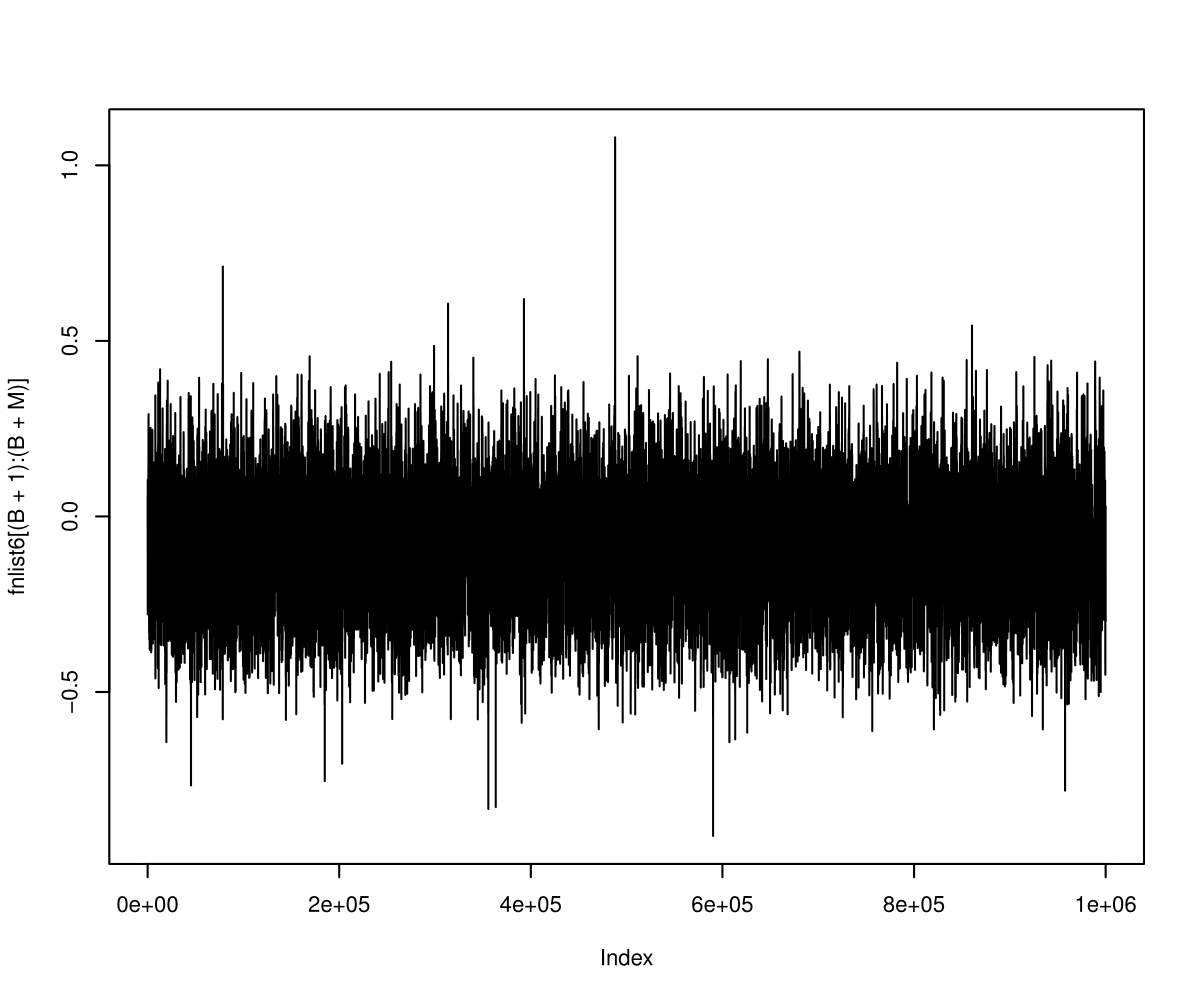
\includegraphics[width=\maxwidth]{figure/p6plot-1} 

\end{knitrout}
		\caption{function values of MCMC algorithm after burning-in}
\end{figure}

From the figure above, we can see that the sample is reasonably well represented (at least the value of the function itself varies significantly around its mean value), indicating a good (accurate) approximation by the MCMC algorithm.

\end{homeworkProblem}

\begin{homeworkProblem}

Consider an independence sampler algorithm on $\chi=(1,\infty)$, where $\pi(x)=5x^{-6}$ and $q(x)=rx^{-r-1}$ for some choice of $r>0$, with identity functional $h(x)=x$. \\
(a) For what value of $r$ will the algorithm provide i.i.d. samples?\\
The algorithm provide i.i.d. samples for $r=5$, because when $r=5$, $\pi(x)=q(x)$. This will eliminate any rejections in the independence sampler, so the sample will be i.i.d.\\\
(b) For what values of $r$ will the sampler be geometrically ergodic?\\
Independence sampler is geometrically ergodic if and only if there is $\delta>0$ such that $q(x)\ge \delta\pi(x)$ for $\pi$-a.e. $x\in \chi$.
With $\chi=(1,\infty)$, we need to be able to pick $\delta>0$ so that 
$$\sup_{x\ge 1}\frac{\pi(x)}{q(x)}=\le \frac{1}{\delta}$$
This means that for any finite $x>1$, we require
$$\frac{pi(x)}{q(x)}=\frac{5x^{-6}}{rx^{-r-1}}=\frac{5}{r}x^{r-5}<\infty$$
So we require $r-5\le 0$, i.e. $r\le 5$. Also since $q(x)=rx^{-r-1}$ is a valid density function, we require $r>0$. Therefore, $r\in(0,5]$.\\
(c) For $r=1/20$, find a number $n$ such that $D(x,n)<0.01$ for all $x\in\chi$.\\
For $r=1/20$, 
$$\frac{\pi(x)}{q(x)}=\frac{5}{\frac{1}{20}}x^{\frac{1}{20}-5}=100x^{-0.99}$$
Therefore, for $x\in\chi=(1,\infty)$, $$\frac{\pi(x)}{q(x)}\le 100$$
so we can pick $\delta=\frac{1}{100}$. Now, as $$D(x,n)\le(1-\delta)^n$$ we can simply choose $n$ such that $(1-\delta)^n<0.01$, so $n>\log(0.01)/\log(0.99)=458.21$. Therefore, $n=459$ will suffice. \\
(d) Write and run a computer program to estimate $\mathbb{E}_\pi(h)$ with this algorithm in the two cases $r=1/20$ and $r=10$, each with $M=10^5$ and $B=10^4$. Estimate the corresponding standard errors by two different methods: (i) using "varfact", and (ii) from repeated independent runs.\\
First, in order to sample from $q(x)$, we notice that if $U~$Uniform(0,1), 
$$P((1-U)^{-\frac{1}{r}\le x}) = P(1-U\ge x^{-r}) = P(U\le 1-x^{-r}) = P(U\le F(x)) = F(x)$$
Therefore, $X=_d(1-U)^{-\frac{1}{r}}$.\\
Then we can implement the independence sampler with the following code:\\
\begin{knitrout}
\definecolor{shadecolor}{rgb}{0.969, 0.969, 0.969}\color{fgcolor}\begin{kframe}
\begin{alltt}
\hlcom{#Estimate E_pi(x) where pi=5x^-6 independence sampler algorithm}
\hlcom{# with proposal distribution q(x) = r x^\{-r-1\}}

\hlstd{h} \hlkwb{=} \hlkwa{function}\hlstd{(}\hlkwc{x}\hlstd{) \{x\}}
\hlstd{g} \hlkwb{=} \hlkwa{function}\hlstd{(}\hlkwc{x}\hlstd{) \{}\hlnum{5}\hlopt{*}\hlstd{x}\hlopt{^}\hlstd{(}\hlopt{-}\hlnum{6}\hlstd{)\}}
\hlstd{q} \hlkwb{=} \hlkwa{function}\hlstd{(}\hlkwc{x}\hlstd{,}\hlkwc{r}\hlstd{) \{r}\hlopt{*}\hlstd{x}\hlopt{^}\hlstd{(}\hlopt{-}\hlstd{r}\hlopt{-}\hlnum{1}\hlstd{)\}}

\hlstd{runs} \hlkwb{=} \hlnum{10}

\hlstd{M} \hlkwb{=} \hlnum{1e+5}
\hlstd{B} \hlkwb{=} \hlnum{1e+4}

\hlstd{funcmean} \hlkwb{=} \hlkwd{numeric}\hlstd{(runs)}
\hlstd{funciidse} \hlkwb{=} \hlkwd{numeric}\hlstd{(runs)}
\hlstd{varfact} \hlkwb{=} \hlkwd{numeric}\hlstd{(runs)}
\hlstd{funcse} \hlkwb{=} \hlkwd{numeric}\hlstd{(runs)}
\hlstd{accrate} \hlkwb{=} \hlkwd{numeric}\hlstd{(runs)}

\hlkwd{cat}\hlstd{(}\hlstr{'B = '}\hlstd{,B,}\hlstr{', M = '}\hlstd{,M,}\hlstr{'\textbackslash{}n'}\hlstd{)}
\hlkwa{for} \hlstd{(i} \hlkwa{in} \hlnum{1}\hlopt{:}\hlstd{runs) \{}
  \hlstd{acc} \hlkwb{=} \hlnum{0}
  \hlstd{fnlist} \hlkwb{=} \hlkwd{numeric}\hlstd{(M}\hlopt{+}\hlstd{B)}
  \hlstd{x} \hlkwb{=} \hlstd{(}\hlnum{1}\hlopt{-}\hlkwd{runif}\hlstd{(}\hlnum{1}\hlstd{))}\hlopt{^}\hlstd{(}\hlopt{-}\hlnum{1}\hlopt{/}\hlstd{r)}
  \hlkwa{for} \hlstd{(j} \hlkwa{in} \hlnum{1}\hlopt{:}\hlstd{(B}\hlopt{+}\hlstd{M)) \{}
    \hlstd{y} \hlkwb{=} \hlstd{(}\hlnum{1}\hlopt{-}\hlkwd{runif}\hlstd{(}\hlnum{1}\hlstd{))}\hlopt{^}\hlstd{(}\hlopt{-}\hlnum{1}\hlopt{/}\hlstd{r)}
    \hlkwa{if} \hlstd{(}\hlkwd{runif}\hlstd{(}\hlnum{1}\hlstd{)}\hlopt{<=}\hlkwd{g}\hlstd{(y)}\hlopt{*}\hlkwd{q}\hlstd{(x,r)}\hlopt{/}\hlkwd{g}\hlstd{(x)}\hlopt{/}\hlkwd{q}\hlstd{(y,r)) \{}
      \hlstd{acc} \hlkwb{=} \hlstd{acc}\hlopt{+}\hlnum{1}
      \hlstd{x} \hlkwb{=} \hlstd{y}
    \hlstd{\}}
    \hlstd{fnlist[j]} \hlkwb{=} \hlkwd{h}\hlstd{(x)}
  \hlstd{\}}

  \hlstd{funcmean[i]} \hlkwb{=} \hlkwd{mean}\hlstd{(fnlist[(B}\hlopt{+}\hlnum{1}\hlstd{)}\hlopt{:}\hlstd{(M}\hlopt{+}\hlstd{B)])}
  \hlstd{funciidse[i]} \hlkwb{=} \hlkwd{sd}\hlstd{(fnlist[(B}\hlopt{+}\hlnum{1}\hlstd{)}\hlopt{:}\hlstd{(M}\hlopt{+}\hlstd{B)])}\hlopt{/}\hlkwd{sqrt}\hlstd{(M)}
  \hlstd{acf_k} \hlkwb{=} \hlkwd{acf}\hlstd{(fnlist[(B}\hlopt{+}\hlnum{1}\hlstd{)}\hlopt{:}\hlstd{(M}\hlopt{+}\hlstd{B)],}\hlkwc{lag.max} \hlstd{=} \hlnum{1000}\hlstd{,}\hlkwc{plot} \hlstd{=} \hlnum{FALSE}\hlstd{)}\hlopt{$}\hlstd{acf}
  \hlstd{varfact[i]} \hlkwb{=} \hlnum{2}\hlopt{*}\hlkwd{sum}\hlstd{(acf_k)}\hlopt{-}\hlnum{1}
  \hlstd{funcse[i]} \hlkwb{=} \hlstd{funciidse[i]}\hlopt{*}\hlkwd{sqrt}\hlstd{(varfact[i])}
  \hlstd{accrate[i]} \hlkwb{=} \hlstd{acc}\hlopt{/}\hlstd{M}

  \hlkwd{cat}\hlstd{(}\hlstr{'Number of samples accepted = '}\hlstd{,acc,}\hlstr{', acceptance rate = '}\hlstd{,accrate[i],}\hlstr{'\textbackslash{}n'}\hlstd{)}
  \hlkwd{cat}\hlstd{(}\hlstr{'Estimate = '}\hlstd{,funcmean[i],}\hlstr{'\textbackslash{}n'}\hlstd{)}
  \hlkwd{cat}\hlstd{(}\hlstr{'i.i.d. standard error = '}\hlstd{,funciidse[i],}\hlstr{'\textbackslash{}n'}\hlstd{)}
  \hlkwd{cat}\hlstd{(}\hlstr{'varfact = '}\hlstd{,varfact[i],}\hlstr{'\textbackslash{}n'}\hlstd{)}
  \hlkwd{cat}\hlstd{(}\hlstr{'Standard error = '}\hlstd{,funcse[i],}\hlstr{'\textbackslash{}n'}\hlstd{)}
\hlstd{\}}
\hlstd{meanse} \hlkwb{<-} \hlkwd{data.frame}\hlstd{(funcmean,funciidse,varfact,funcse,accrate)}
\hlstd{estse} \hlkwb{=} \hlkwd{sd}\hlstd{(funcmean)}
\hlkwd{cat}\hlstd{(}\hlstr{'Standard error calculated from multiple runs = '}\hlstd{,estse,}\hlstr{'\textbackslash{}n'}\hlstd{)}
\end{alltt}
\end{kframe}
\end{knitrout}
with $r=1/20$, the output of running the program is printed below:

\begin{knitrout}
\definecolor{shadecolor}{rgb}{0.969, 0.969, 0.969}\color{fgcolor}\begin{kframe}
\begin{verbatim}
## B =  10000 , M =  1e+05
## Number of samples accepted =  2093 , acceptance rate =  0.02093 
## Estimate =  1.238635 
## i.i.d. standard error =  0.0009258633 
## varfact =  114.0854 
## Standard error =  0.009889218 
## Number of samples accepted =  2180 , acceptance rate =  0.0218 
## Estimate =  1.237005 
## i.i.d. standard error =  0.0009949706 
## varfact =  72.25659 
## Standard error =  0.008457635 
## Number of samples accepted =  2203 , acceptance rate =  0.02203 
## Estimate =  1.243761 
## i.i.d. standard error =  0.0009788405 
## varfact =  91.95337 
## Standard error =  0.009386328 
## Number of samples accepted =  2205 , acceptance rate =  0.02205 
## Estimate =  1.26803 
## i.i.d. standard error =  0.001196367 
## varfact =  114.8249 
## Standard error =  0.01281984 
## Number of samples accepted =  2239 , acceptance rate =  0.02239 
## Estimate =  1.26214 
## i.i.d. standard error =  0.001043855 
## varfact =  132.7526 
## Standard error =  0.01202712 
## Number of samples accepted =  2237 , acceptance rate =  0.02237 
## Estimate =  1.240768 
## i.i.d. standard error =  0.0009611 
## varfact =  65.51433 
## Standard error =  0.007779232 
## Number of samples accepted =  2167 , acceptance rate =  0.02167 
## Estimate =  1.259207 
## i.i.d. standard error =  0.001016062 
## varfact =  108.19 
## Standard error =  0.01056851 
## Number of samples accepted =  2188 , acceptance rate =  0.02188 
## Estimate =  1.250411 
## i.i.d. standard error =  0.001161109 
## varfact =  89.67467 
## Standard error =  0.01099532 
## Number of samples accepted =  2165 , acceptance rate =  0.02165 
## Estimate =  1.25477 
## i.i.d. standard error =  0.001067317 
## varfact =  103.8663 
## Standard error =  0.01087754 
## Number of samples accepted =  2212 , acceptance rate =  0.02212 
## Estimate =  1.252788 
## i.i.d. standard error =  0.001087062 
## varfact =  108.7818 
## Standard error =  0.01133789
## Standard error calculated from multiple runs =  0.01056452
\end{verbatim}
\end{kframe}
\end{knitrout}



with $r=10$, the output of running the program is printed below:

\begin{knitrout}
\definecolor{shadecolor}{rgb}{0.969, 0.969, 0.969}\color{fgcolor}\begin{kframe}
\begin{verbatim}
## B =  10000 , M =  1e+05
## Number of samples accepted =  73929 , acceptance rate =  0.73929 
## Estimate =  1.24135 
## i.i.d. standard error =  0.0009011254 
## varfact =  46.05885 
## Standard error =  0.006115638 
## Number of samples accepted =  74109 , acceptance rate =  0.74109 
## Estimate =  1.227835 
## i.i.d. standard error =  0.0007831439 
## varfact =  20.71352 
## Standard error =  0.003564253 
## Number of samples accepted =  73333 , acceptance rate =  0.73333 
## Estimate =  1.245432 
## i.i.d. standard error =  0.000920215 
## varfact =  101.153 
## Standard error =  0.009255046 
## Number of samples accepted =  74465 , acceptance rate =  0.74465 
## Estimate =  1.233405 
## i.i.d. standard error =  0.0008525449 
## varfact =  42.70032 
## Standard error =  0.005570996 
## Number of samples accepted =  73682 , acceptance rate =  0.73682 
## Estimate =  1.24653 
## i.i.d. standard error =  0.0009628246 
## varfact =  124.5792 
## Standard error =  0.01074657 
## Number of samples accepted =  73657 , acceptance rate =  0.73657 
## Estimate =  1.239802 
## i.i.d. standard error =  0.0009025768 
## varfact =  124.087 
## Standard error =  0.0100542 
## Number of samples accepted =  73517 , acceptance rate =  0.73517 
## Estimate =  1.244985 
## i.i.d. standard error =  0.0009591974 
## varfact =  177.6196 
## Standard error =  0.01278361 
## Number of samples accepted =  73592 , acceptance rate =  0.73592 
## Estimate =  1.246485 
## i.i.d. standard error =  0.0009477594 
## varfact =  51.65175 
## Standard error =  0.006811466 
## Number of samples accepted =  73218 , acceptance rate =  0.73218 
## Estimate =  1.247764 
## i.i.d. standard error =  0.0009336237 
## varfact =  37.46121 
## Standard error =  0.005714297 
## Number of samples accepted =  73434 , acceptance rate =  0.73434 
## Estimate =  1.24259 
## i.i.d. standard error =  0.0008906098 
## varfact =  60.98202 
## Standard error =  0.00695486
## Standard error calculated from multiple runs =  0.00643962
\end{verbatim}
\end{kframe}
\end{knitrout}


For ease of reading the result, we tabulate the result in the following two tables\\
\begin{center}
\begin{knitrout}
\definecolor{shadecolor}{rgb}{0.969, 0.969, 0.969}\color{fgcolor}
\begin{tabular}{r|r|r|r|r}
\hline
funcmean & funciidse & varfact & funcse & accrate\\
\hline
1.238635 & 0.0009259 & 114.08541 & 0.0098892 & 0.02093\\
\hline
1.237005 & 0.0009950 & 72.25659 & 0.0084576 & 0.02180\\
\hline
1.243761 & 0.0009788 & 91.95337 & 0.0093863 & 0.02203\\
\hline
1.268030 & 0.0011964 & 114.82491 & 0.0128198 & 0.02205\\
\hline
1.262140 & 0.0010439 & 132.75263 & 0.0120271 & 0.02239\\
\hline
1.240768 & 0.0009611 & 65.51433 & 0.0077792 & 0.02237\\
\hline
1.259207 & 0.0010161 & 108.18999 & 0.0105685 & 0.02167\\
\hline
1.250411 & 0.0011611 & 89.67467 & 0.0109953 & 0.02188\\
\hline
1.254770 & 0.0010673 & 103.86630 & 0.0108775 & 0.02165\\
\hline
1.252789 & 0.0010871 & 108.78176 & 0.0113379 & 0.02212\\
\hline
\end{tabular}


\end{knitrout}
for r=1/20
\end{center}
mean of estimate = 1.2507516\\
mean of estimate standard error = 0.0104139\\
standard deviation calculated from multiple runs = 0.0015607\\
mean of acceptance rate = 0.021889\\
\begin{center}
\begin{knitrout}
\definecolor{shadecolor}{rgb}{0.969, 0.969, 0.969}\color{fgcolor}
\begin{tabular}{r|r|r|r|r}
\hline
funcmean & funciidse & varfact & funcse & accrate\\
\hline
1.241350 & 0.0009011 & 46.05885 & 0.0061156 & 0.73929\\
\hline
1.227835 & 0.0007831 & 20.71352 & 0.0035643 & 0.74109\\
\hline
1.245432 & 0.0009202 & 101.15297 & 0.0092550 & 0.73333\\
\hline
1.233405 & 0.0008525 & 42.70032 & 0.0055710 & 0.74465\\
\hline
1.246530 & 0.0009628 & 124.57925 & 0.0107466 & 0.73682\\
\hline
1.239802 & 0.0009026 & 124.08702 & 0.0100542 & 0.73657\\
\hline
1.244985 & 0.0009592 & 177.61965 & 0.0127836 & 0.73517\\
\hline
1.246485 & 0.0009478 & 51.65175 & 0.0068115 & 0.73592\\
\hline
1.247764 & 0.0009336 & 37.46121 & 0.0057143 & 0.73218\\
\hline
1.242590 & 0.0008906 & 60.98202 & 0.0069549 & 0.73434\\
\hline
\end{tabular}


\end{knitrout}
for r=10
\end{center}
mean of estimate = 1.2416177\\
mean of estimate standard error = 0.0077571\\
standard deviation calculated from multiple runs = 0.002838\\
mean of acceptance rate = 0.736936\\
(e) First notice that the standard error calculated from varfact and i.i.d standard error is slightly larger than the standard error calculated from multiple runs in both cases. Also notice that the two estimates are quite close to each other, and the standar errors are also quite similar in the cases where $r=1/20$ and $r=10$. This result is quite surprising because the acceptance rate for the two cases are completely different. For $r=1/20$, the acceptance rate is just over 0.02, where as the acceptance rate is about 0.73 for the $r=10$ case.\\
Also, for $r=1/20$ the sampler is geometrially ergodic and should be more reliable, at least to the extend that we know the Central Limit Theorem will hold for sure.\\
Finally, we can analytically calculate the mean and standard deviation 
\begin{align*}
\mathbb{E}_\pi h &= \int_1^\infty 5x^{-5}dx = -\frac{5}{4}x^{-4}\bigg|^\infty_1 = \frac{5}{4}\\
\mathbb{E}_\pi h^2 &= \int_1^\infty 5x^{-4}dx = -\frac{5}{3}x^{-3}\bigg|^\infty_1 = \frac{5}{3}\\
\sigma &= \sqrt{\frac{5}{3}-\left(\frac{5}{4}\right)^2}=0.3227\\
\frac{\sigma}{\sqrt{M}} &\approx 0.001
\end{align*}
Both 95\% confidence intervals contain the exacty value. 

\end{homeworkProblem}

\begin{homeworkProblem}

Let $\chi = \mathbb{R}$, and let $\pi(x)=cg(x)$, where $g(x)=e^{-|x|/10}(1+\cos(x)\sin(x))$, and let $h(x)=x+x^2$. With appropriate choise of $M,B, \sigma$, and starting distribution $\mathcal{L}(X_0)$, estimate $\mathbb{E}_\pi(h)$ in each of the two different ways:
(a) With a usual random-walk Metropolis algorithm for $\pi$, with the usual proposal distribution $Y_n$~$N(X_{n-1},\sigma^2)$.
For this problem, we choose again $M$ to be 10e+6 and $B$ to be 10e+5, and we choose $\sigma$ to be 53 so that the acceptance rate is around the optimal value 0.234.
The RWM algorithm is implemented using the following code:
\begin{knitrout}
\definecolor{shadecolor}{rgb}{0.969, 0.969, 0.969}\color{fgcolor}\begin{kframe}
\begin{alltt}
\hlcom{#Estimate E_pi(X+X^2) where pi=cg using RWM algorithm where}
\hlcom{# g(x) = e^(-|x|/10)*(1+cos(x)sin(x^3))}
\hlcom{# with increments following a N(0,sigma^2) distribution}

\hlstd{fn} \hlkwb{=} \hlkwa{function}\hlstd{(}\hlkwc{x}\hlstd{) \{x}\hlopt{+}\hlstd{x}\hlopt{^}\hlnum{2}\hlstd{\}}
\hlstd{g} \hlkwb{=} \hlkwa{function}\hlstd{(}\hlkwc{x}\hlstd{) \{}\hlkwd{exp}\hlstd{(}\hlopt{-}\hlkwd{abs}\hlstd{(x)}\hlopt{/}\hlnum{10}\hlstd{)}\hlopt{*}\hlstd{(}\hlnum{1}\hlopt{+}\hlkwd{cos}\hlstd{(x)}\hlopt{*}\hlkwd{sin}\hlstd{(x}\hlopt{^}\hlnum{3}\hlstd{))\}}

\hlstd{sigma} \hlkwb{=} \hlnum{53}
\hlstd{M} \hlkwb{=} \hlnum{1e+6}
\hlstd{B} \hlkwb{=} \hlnum{1e+5}

\hlcom{#initialization}
\hlstd{fnlist} \hlkwb{=} \hlkwd{numeric}\hlstd{(M}\hlopt{+}\hlstd{B)}
\hlstd{xlist} \hlkwb{=} \hlkwd{numeric}\hlstd{(M}\hlopt{+}\hlstd{B)}
\hlstd{x} \hlkwb{=} \hlkwd{rnorm}\hlstd{(}\hlnum{1}\hlstd{,}\hlnum{0}\hlstd{,sigma)}
\hlstd{acc} \hlkwb{=} \hlnum{0}

\hlkwa{for} \hlstd{(i} \hlkwa{in} \hlnum{1}\hlopt{:}\hlstd{(M}\hlopt{+}\hlstd{B)) \{}
  \hlstd{eps} \hlkwb{=} \hlkwd{rnorm}\hlstd{(}\hlnum{1}\hlstd{,}\hlnum{0}\hlstd{,sigma)}

  \hlkwa{if} \hlstd{(}\hlkwd{runif}\hlstd{(}\hlnum{1}\hlstd{)}\hlopt{<=}\hlkwd{g}\hlstd{(x}\hlopt{+}\hlstd{eps)}\hlopt{/}\hlkwd{g}\hlstd{(x)) \{}
    \hlkwa{if} \hlstd{(i}\hlopt{>}\hlstd{B)}
      \hlstd{acc}\hlkwb{=}\hlstd{acc}\hlopt{+}\hlnum{1}
    \hlstd{x} \hlkwb{=} \hlstd{x}\hlopt{+}\hlstd{eps}
  \hlstd{\}}
  \hlstd{xlist[i]} \hlkwb{=} \hlstd{x}
  \hlstd{fnlist[i]} \hlkwb{=} \hlkwd{fn}\hlstd{(x)}
\hlstd{\}}

\hlstd{funcmean} \hlkwb{=} \hlkwd{mean}\hlstd{(fnlist[(B}\hlopt{+}\hlnum{1}\hlstd{)}\hlopt{:}\hlstd{(M}\hlopt{+}\hlstd{B)])}
\hlstd{funciidse} \hlkwb{=} \hlkwd{sd}\hlstd{(fnlist[(B}\hlopt{+}\hlnum{1}\hlstd{)}\hlopt{:}\hlstd{(M}\hlopt{+}\hlstd{B)])}\hlopt{/}\hlkwd{sqrt}\hlstd{(M)}
\hlstd{acf_k} \hlkwb{=} \hlkwd{acf}\hlstd{(fnlist[(B}\hlopt{+}\hlnum{1}\hlstd{)}\hlopt{:}\hlstd{(M}\hlopt{+}\hlstd{B)],}\hlkwc{lag.max} \hlstd{=} \hlnum{1000}\hlstd{,}\hlkwc{plot} \hlstd{=} \hlnum{FALSE}\hlstd{)}\hlopt{$}\hlstd{acf}
\hlstd{varfact} \hlkwb{=} \hlnum{2}\hlopt{*}\hlkwd{sum}\hlstd{(acf_k[}\hlnum{1}\hlopt{:}\hlkwd{min}\hlstd{(}\hlkwd{which}\hlstd{(acf_k}\hlopt{<}\hlnum{0.05}\hlstd{))])}\hlopt{-}\hlnum{1}
\hlstd{funcse} \hlkwb{=} \hlstd{funciidse}\hlopt{*}\hlkwd{sqrt}\hlstd{(varfact)}
\hlstd{accrate} \hlkwb{=} \hlstd{acc}\hlopt{/}\hlstd{M}

\hlkwd{cat}\hlstd{(}\hlstr{'B = '}\hlstd{,B,}\hlstr{', M = '}\hlstd{,M,}\hlstr{'\textbackslash{}n'}\hlstd{)}
\hlkwd{cat}\hlstd{(}\hlstr{'Number of samples accepted = '}\hlstd{,acc,}\hlstr{', acceptance rate = '}\hlstd{,accrate,}\hlstr{'\textbackslash{}n'}\hlstd{)}
\hlkwd{cat}\hlstd{(}\hlstr{'Estimate = '}\hlstd{,funcmean,}\hlstr{'\textbackslash{}n'}\hlstd{)}
\hlkwd{cat}\hlstd{(}\hlstr{'i.i.d. standard error = '}\hlstd{,funciidse,}\hlstr{'\textbackslash{}n'}\hlstd{)}
\hlkwd{cat}\hlstd{(}\hlstr{'varfact = '}\hlstd{,varfact,}\hlstr{'\textbackslash{}n'}\hlstd{)}
\hlkwd{cat}\hlstd{(}\hlstr{'Standard error = '}\hlstd{,funcse,}\hlstr{'\textbackslash{}n'}\hlstd{)}
\end{alltt}
\end{kframe}
\end{knitrout}
Output of several runs:
\begin{knitrout}
\definecolor{shadecolor}{rgb}{0.969, 0.969, 0.969}\color{fgcolor}\begin{kframe}
\begin{verbatim}
## B =  1e+05 , M =  1e+06 
## Number of samples accepted =  238066 , acceptance rate =  0.238066 
## Estimate =  200.6944 
## i.i.d. standard error =  0.4448528 
## varfact =  6.844363 
## Standard error =  1.163812
## B =  1e+05 , M =  1e+06 
## Number of samples accepted =  237394 , acceptance rate =  0.237394 
## Estimate =  199.571 
## i.i.d. standard error =  0.4484531 
## varfact =  6.913195 
## Standard error =  1.179116
## B =  1e+05 , M =  1e+06 
## Number of samples accepted =  238054 , acceptance rate =  0.238054 
## Estimate =  200.1975 
## i.i.d. standard error =  0.4433383 
## varfact =  6.77882 
## Standard error =  1.154283
## B =  1e+05 , M =  1e+06 
## Number of samples accepted =  238477 , acceptance rate =  0.238477 
## Estimate =  200.3298 
## i.i.d. standard error =  0.4522812 
## varfact =  7.017603 
## Standard error =  1.198127
## B =  1e+05 , M =  1e+06 
## Number of samples accepted =  237175 , acceptance rate =  0.237175 
## Estimate =  198.6471 
## i.i.d. standard error =  0.4413461 
## varfact =  6.776058 
## Standard error =  1.148862
\end{verbatim}
\end{kframe}
\end{knitrout}
The tabulated result is as follows:\\
\begin{center}
\begin{knitrout}
\definecolor{shadecolor}{rgb}{0.969, 0.969, 0.969}\color{fgcolor}
\begin{tabular}{r|r|r|r|r}
\hline
estimation & acc\_rate & seiid & varfact & standard\_error\\
\hline
200.6944 & 0.238066 & 0.4448528 & 6.776058 & 1.163812\\
\hline
199.5710 & 0.237394 & 0.4484531 & 6.776058 & 1.179116\\
\hline
200.1975 & 0.238054 & 0.4433383 & 6.776058 & 1.154283\\
\hline
200.3298 & 0.238477 & 0.4522812 & 6.776058 & 1.198127\\
\hline
198.6471 & 0.237175 & 0.4413461 & 6.776058 & 1.148862\\
\hline
\end{tabular}


\end{knitrout}
\end{center}
We notice that the varfact values are quite small, indicating that the samples are not strongly correlated. To verify the effectiveness of the sampler, here we plot the value of $x$ after the burn-in stage
\begin{figure}[H]
  \centering
\begin{knitrout}
\definecolor{shadecolor}{rgb}{0.969, 0.969, 0.969}\color{fgcolor}\begin{kframe}
\begin{alltt}
\hlstd{xlist8a} \hlkwb{=} \hlstd{xlist}
\hlkwd{plot}\hlstd{(xlist8a[(B}\hlopt{+}\hlnum{1}\hlstd{)}\hlopt{:}\hlstd{(B}\hlopt{+}\hlstd{M)],}\hlkwc{type}\hlstd{=}\hlstr{'l'}\hlstd{)}
\end{alltt}
\end{kframe}
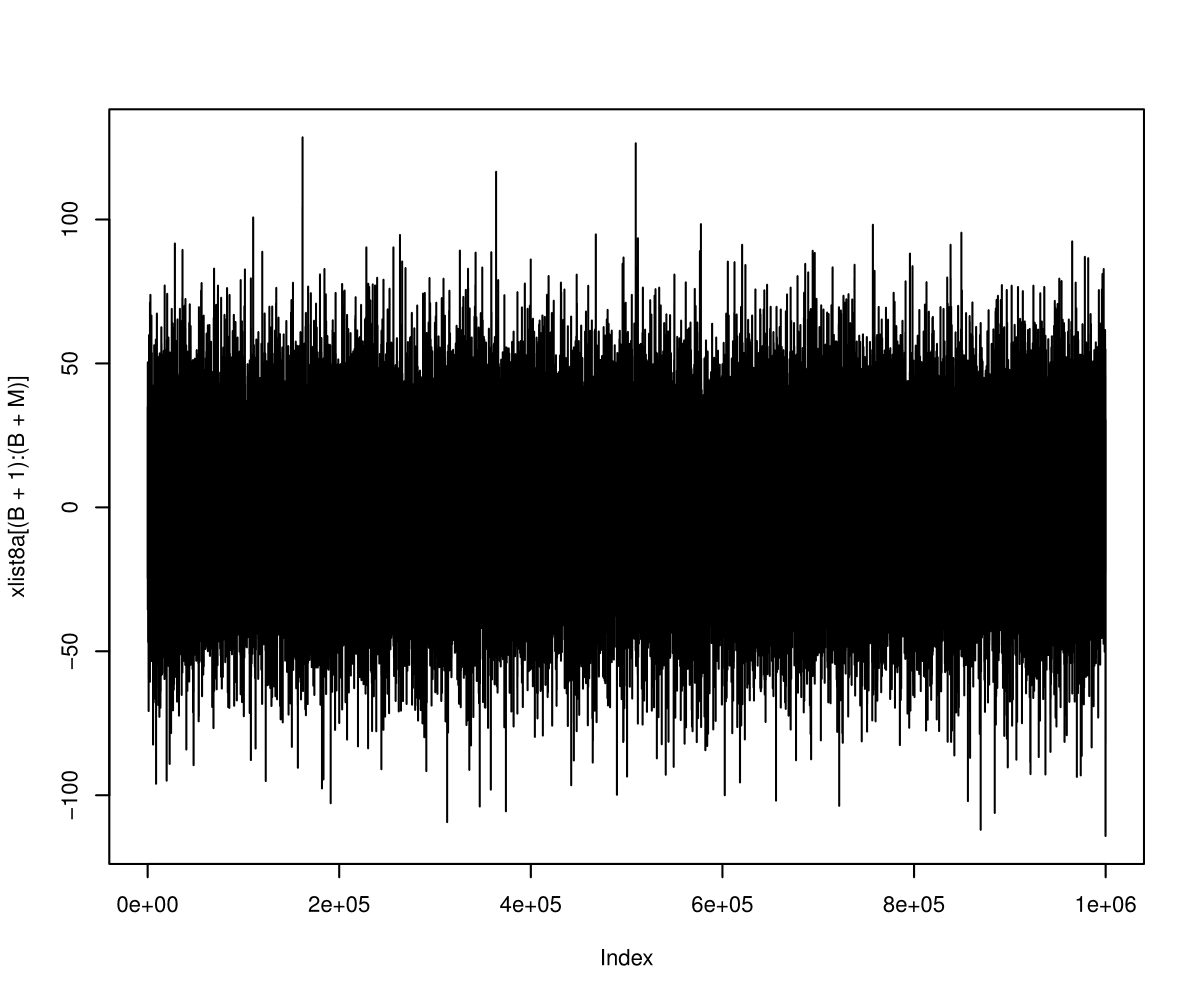
\includegraphics[width=\maxwidth]{figure/p8aplot-1} 

\end{knitrout}
		\caption{$x$ values of RWM algorithm after burning-in}
\end{figure}
From the figure above, we can see that the sample is reasonably well represented because of the high variability and low correlation, indicating a good (accurate) approximation by the RWM algorithm.\\


(b) With a Langevin (Metropolis-Hastings) algorithm with proposals $Y_n$~$N(X_{n-1}+\frac{1}{2}\sigma^2g'(X_{n-1})/g(X_{n-1}),\sigma^2)$.
First we calculate analycically $g'(x)$:
\begin{align*}
\frac{dg}{dx} &= 
\begin{cases}
  \frac{d}{dx}\left(e^{-x/10}(1+\cos(x)\sin(x^3))\right) &\text{for }x>0\\
  \frac{d}{dx}\left(e^{x/10}(1+\cos(x)\sin(x^3))\right) &\text{for }x<0
\end{cases}\\
  &=\begin{cases}
  -\frac{1}{10}e^{-x/10}(1+\cos(x)\sin(x^3)) +e^{-x/10}(3x^2\cos(x)\cos(x^3)-\sin(x)\sin(x^3)) &\text{for }x>0\\
  \frac{1}{10}e^{x/10}(1+\cos(x)\sin(x^3)) +e^{x/10}(3x^2\cos(x)\cos(x^3)-\sin(x)\sin(x^3)) &\text{for }x<0\\
  \end{cases}
\end{align*}
With the closed form of $g'(x)$ calculated, we can implement the Langevin algorithm with the following code
\begin{knitrout}
\definecolor{shadecolor}{rgb}{0.969, 0.969, 0.969}\color{fgcolor}\begin{kframe}
\begin{alltt}
\hlcom{#Estimate E_pi(X+X^2) where pi=cg using Metropolis-Hasting algorithm where}
\hlcom{# g(x) = e^(-|x|/10)*(1+cos(x)sin(x^3))}
\hlcom{# with proposal N(X_(n-1)+1/2sigma^2g'(X_(n-1)),sigma^2)}

\hlstd{sigma} \hlkwb{=} \hlnum{0.1}
\hlstd{M} \hlkwb{=}\hlnum{1e5}
\hlstd{B} \hlkwb{=} \hlnum{2e4}

\hlstd{fn} \hlkwb{=} \hlkwa{function}\hlstd{(}\hlkwc{x}\hlstd{) \{x}\hlopt{+}\hlstd{x}\hlopt{^}\hlnum{2}\hlstd{\}}
\hlstd{g} \hlkwb{=} \hlkwa{function}\hlstd{(}\hlkwc{x}\hlstd{) \{}\hlkwd{exp}\hlstd{(}\hlopt{-}\hlkwd{abs}\hlstd{(x)}\hlopt{/}\hlnum{10}\hlstd{)}\hlopt{*}\hlstd{(}\hlnum{1}\hlopt{+}\hlkwd{cos}\hlstd{(x)}\hlopt{*}\hlkwd{sin}\hlstd{(x}\hlopt{^}\hlnum{3}\hlstd{))\}}
\hlstd{gp} \hlkwb{=} \hlkwa{function}\hlstd{(}\hlkwc{x}\hlstd{) \{}
  \hlkwa{if} \hlstd{(x}\hlopt{>=}\hlnum{0}\hlstd{)}
    \hlopt{-}\hlkwd{exp}\hlstd{(}\hlopt{-}\hlstd{x}\hlopt{/}\hlnum{10}\hlstd{)}\hlopt{/}\hlnum{10}\hlopt{*}\hlstd{(}\hlnum{1}\hlopt{+}\hlkwd{cos}\hlstd{(x)}\hlopt{*}\hlkwd{sin}\hlstd{(x}\hlopt{^}\hlnum{3}\hlstd{))}\hlopt{+}\hlkwd{exp}\hlstd{(}\hlopt{-}\hlstd{x}\hlopt{/}\hlnum{10}\hlstd{)}\hlopt{*}\hlstd{(}\hlnum{3}\hlopt{*}\hlstd{x}\hlopt{^}\hlnum{2}\hlopt{*}\hlkwd{cos}\hlstd{(x)}\hlopt{*}\hlkwd{cos}\hlstd{(x}\hlopt{^}\hlnum{3}\hlstd{)}\hlopt{-}\hlkwd{sin}\hlstd{(x)}\hlopt{*}\hlkwd{sin}\hlstd{(x}\hlopt{^}\hlnum{3}\hlstd{))}
  \hlkwa{else}
    \hlkwd{exp}\hlstd{(x}\hlopt{/}\hlnum{10}\hlstd{)}\hlopt{/}\hlnum{10}\hlopt{*}\hlstd{(}\hlnum{1}\hlopt{+}\hlkwd{cos}\hlstd{(x)}\hlopt{*}\hlkwd{sin}\hlstd{(x}\hlopt{^}\hlnum{3}\hlstd{))}\hlopt{+}\hlkwd{exp}\hlstd{(x}\hlopt{/}\hlnum{10}\hlstd{)}\hlopt{*}\hlstd{(}\hlnum{3}\hlopt{*}\hlstd{x}\hlopt{^}\hlnum{2}\hlopt{*}\hlkwd{cos}\hlstd{(x)}\hlopt{*}\hlkwd{cos}\hlstd{(x}\hlopt{^}\hlnum{3}\hlstd{)}\hlopt{-}\hlkwd{sin}\hlstd{(x)}\hlopt{*}\hlkwd{sin}\hlstd{(x}\hlopt{^}\hlnum{3}\hlstd{))}
\hlstd{\}}
\hlstd{qq} \hlkwb{=} \hlkwa{function}\hlstd{(}\hlkwc{x}\hlstd{,}\hlkwc{y}\hlstd{) \{}
  \hlkwd{exp}\hlstd{(}\hlopt{-}\hlstd{(y}\hlopt{-}\hlstd{x}\hlopt{-}\hlstd{sigma}\hlopt{^}\hlnum{2}\hlopt{*}\hlkwd{gp}\hlstd{(x)}\hlopt{/}\hlkwd{g}\hlstd{(x)}\hlopt{/}\hlnum{2}\hlstd{)}\hlopt{^}\hlnum{2}\hlopt{/}\hlstd{sigma}\hlopt{^}\hlnum{2}\hlopt{/}\hlnum{2}\hlstd{)}
\hlstd{\}}

\hlcom{#initialization}
\hlstd{fnlist} \hlkwb{=} \hlkwd{numeric}\hlstd{(M}\hlopt{+}\hlstd{B)}
\hlstd{xlist} \hlkwb{=} \hlkwd{numeric}\hlstd{(M}\hlopt{+}\hlstd{B)}
\hlstd{x} \hlkwb{=} \hlkwd{rnorm}\hlstd{(}\hlnum{1}\hlstd{,}\hlnum{0}\hlstd{,sigma)}
\hlstd{acc} \hlkwb{=} \hlnum{0}

\hlkwa{for} \hlstd{(i} \hlkwa{in} \hlnum{1}\hlopt{:}\hlstd{(M}\hlopt{+}\hlstd{B)) \{}

  \hlstd{m} \hlkwb{=} \hlnum{1}\hlopt{/}\hlnum{2}\hlopt{*}\hlstd{sigma}\hlopt{^}\hlnum{2}\hlopt{*}\hlkwd{gp}\hlstd{(x)}\hlopt{/}\hlkwd{g}\hlstd{(x)}
  \hlstd{y} \hlkwb{=} \hlkwd{rnorm}\hlstd{(}\hlnum{1}\hlstd{,x}\hlopt{+}\hlstd{m,sigma)}

  \hlkwa{if} \hlstd{(}\hlkwd{runif}\hlstd{(}\hlnum{1}\hlstd{)}\hlopt{<=}\hlkwd{g}\hlstd{(y)}\hlopt{*}\hlkwd{qq}\hlstd{(y,x)}\hlopt{/}\hlkwd{g}\hlstd{(x)}\hlopt{/}\hlkwd{qq}\hlstd{(x,y)) \{}
    \hlkwa{if} \hlstd{(i}\hlopt{>}\hlstd{B)}
      \hlstd{acc}\hlkwb{=}\hlstd{acc}\hlopt{+}\hlnum{1}
    \hlstd{x} \hlkwb{=} \hlstd{y}
  \hlstd{\}}
  \hlstd{xlist[i]} \hlkwb{=} \hlstd{x}
  \hlstd{fnlist[i]} \hlkwb{=} \hlkwd{fn}\hlstd{(x)}
\hlstd{\}}

\hlstd{funcmean} \hlkwb{=} \hlkwd{mean}\hlstd{(fnlist[(B}\hlopt{+}\hlnum{1}\hlstd{)}\hlopt{:}\hlstd{(M}\hlopt{+}\hlstd{B)])}
\hlstd{funciidse} \hlkwb{=} \hlkwd{sd}\hlstd{(fnlist[(B}\hlopt{+}\hlnum{1}\hlstd{)}\hlopt{:}\hlstd{(M}\hlopt{+}\hlstd{B)])}\hlopt{/}\hlkwd{sqrt}\hlstd{(M)}
\hlstd{acf_k} \hlkwb{=} \hlkwd{acf}\hlstd{(fnlist[(B}\hlopt{+}\hlnum{1}\hlstd{)}\hlopt{:}\hlstd{(M}\hlopt{+}\hlstd{B)],}\hlkwc{lag.max} \hlstd{=} \hlnum{1000}\hlstd{,}\hlkwc{plot} \hlstd{=} \hlnum{FALSE}\hlstd{)}\hlopt{$}\hlstd{acf}
\hlstd{varfact} \hlkwb{=} \hlnum{2}\hlopt{*}\hlkwd{sum}\hlstd{(acf_k)}\hlopt{-}\hlnum{1}
\hlstd{funcse} \hlkwb{=} \hlstd{funciidse}\hlopt{*}\hlkwd{sqrt}\hlstd{(varfact)}
\hlstd{accrate} \hlkwb{=} \hlstd{acc}\hlopt{/}\hlstd{M}

\hlkwd{cat}\hlstd{(}\hlstr{'B = '}\hlstd{,B,}\hlstr{', M = '}\hlstd{,M,}\hlstr{'\textbackslash{}n'}\hlstd{)}
\hlkwd{cat}\hlstd{(}\hlstr{'Number of samples accepted = '}\hlstd{,acc,}\hlstr{', acceptance rate = '}\hlstd{,accrate,}\hlstr{'\textbackslash{}n'}\hlstd{)}
\hlkwd{cat}\hlstd{(}\hlstr{'Estimate = '}\hlstd{,funcmean,}\hlstr{'\textbackslash{}n'}\hlstd{)}
\hlkwd{cat}\hlstd{(}\hlstr{'i.i.d. standard error = '}\hlstd{,funciidse,}\hlstr{'\textbackslash{}n'}\hlstd{)}
\hlkwd{cat}\hlstd{(}\hlstr{'varfact = '}\hlstd{,varfact,}\hlstr{'\textbackslash{}n'}\hlstd{)}
\hlkwd{cat}\hlstd{(}\hlstr{'Standard error = '}\hlstd{,funcse,}\hlstr{'\textbackslash{}n'}\hlstd{)}
\end{alltt}
\end{kframe}
\end{knitrout}
Output of several runs:
\begin{knitrout}
\definecolor{shadecolor}{rgb}{0.969, 0.969, 0.969}\color{fgcolor}\begin{kframe}
\begin{verbatim}
## B =  20000 , M =  1e+05 
## Number of samples accepted =  72892 , acceptance rate =  0.72892 
## Estimate =  16.37651 
## i.i.d. standard error =  0.07014971 
## varfact =  1875.972 
## Standard error =  3.038359
## B =  20000 , M =  1e+05 
## Number of samples accepted =  66806 , acceptance rate =  0.66806 
## Estimate =  51.28206 
## i.i.d. standard error =  0.2649013 
## varfact =  1958.284 
## Standard error =  11.72255
## B =  20000 , M =  1e+05 
## Number of samples accepted =  55956 , acceptance rate =  0.55956 
## Estimate =  23.24639 
## i.i.d. standard error =  0.06920837 
## varfact =  1798.478 
## Standard error =  2.935021
## B =  20000 , M =  1e+05 
## Number of samples accepted =  64279 , acceptance rate =  0.64279 
## Estimate =  18.73548 
## i.i.d. standard error =  0.06656209 
## varfact =  1821.751 
## Standard error =  2.841001
## B =  20000 , M =  1e+05 
## Number of samples accepted =  76744 , acceptance rate =  0.76744 
## Estimate =  8.867096 
## i.i.d. standard error =  0.03519465 
## varfact =  1715.128 
## Standard error =  1.457555
\end{verbatim}
\end{kframe}
\end{knitrout}
The tabulated result is as follows:\\
\begin{center}
\begin{knitrout}
\definecolor{shadecolor}{rgb}{0.969, 0.969, 0.969}\color{fgcolor}
\begin{tabular}{r|r|r|r|r}
\hline
estimation & acc\_rate & seiid & varfact\_r & standard\_error\\
\hline
16.376511 & 0.72892 & 0.0701497 & 1875.972 & 3.038359\\
\hline
51.282063 & 0.66806 & 0.2649013 & 1958.284 & 11.722547\\
\hline
23.246395 & 0.55956 & 0.0692084 & 1798.478 & 2.935021\\
\hline
18.735479 & 0.64279 & 0.0665621 & 1821.751 & 2.841001\\
\hline
8.867096 & 0.76744 & 0.0351946 & 1715.128 & 1.457555\\
\hline
\end{tabular}


\end{knitrout}
\end{center}
We notice that the varfact values are quite small, indicating that the samples are not strongly correlated. To verify the effectiveness of the sampler, here we plot the value of $x$ after the burn-in stage
\begin{figure}[H]
  \centering
\begin{knitrout}
\definecolor{shadecolor}{rgb}{0.969, 0.969, 0.969}\color{fgcolor}\begin{kframe}
\begin{alltt}
\hlstd{xlist8b} \hlkwb{=} \hlstd{xlist}
\hlkwd{plot}\hlstd{(xlist8b[(B}\hlopt{+}\hlnum{1}\hlstd{)}\hlopt{:}\hlstd{(B}\hlopt{+}\hlstd{M)],}\hlkwc{type}\hlstd{=}\hlstr{'l'}\hlstd{)}
\end{alltt}
\end{kframe}
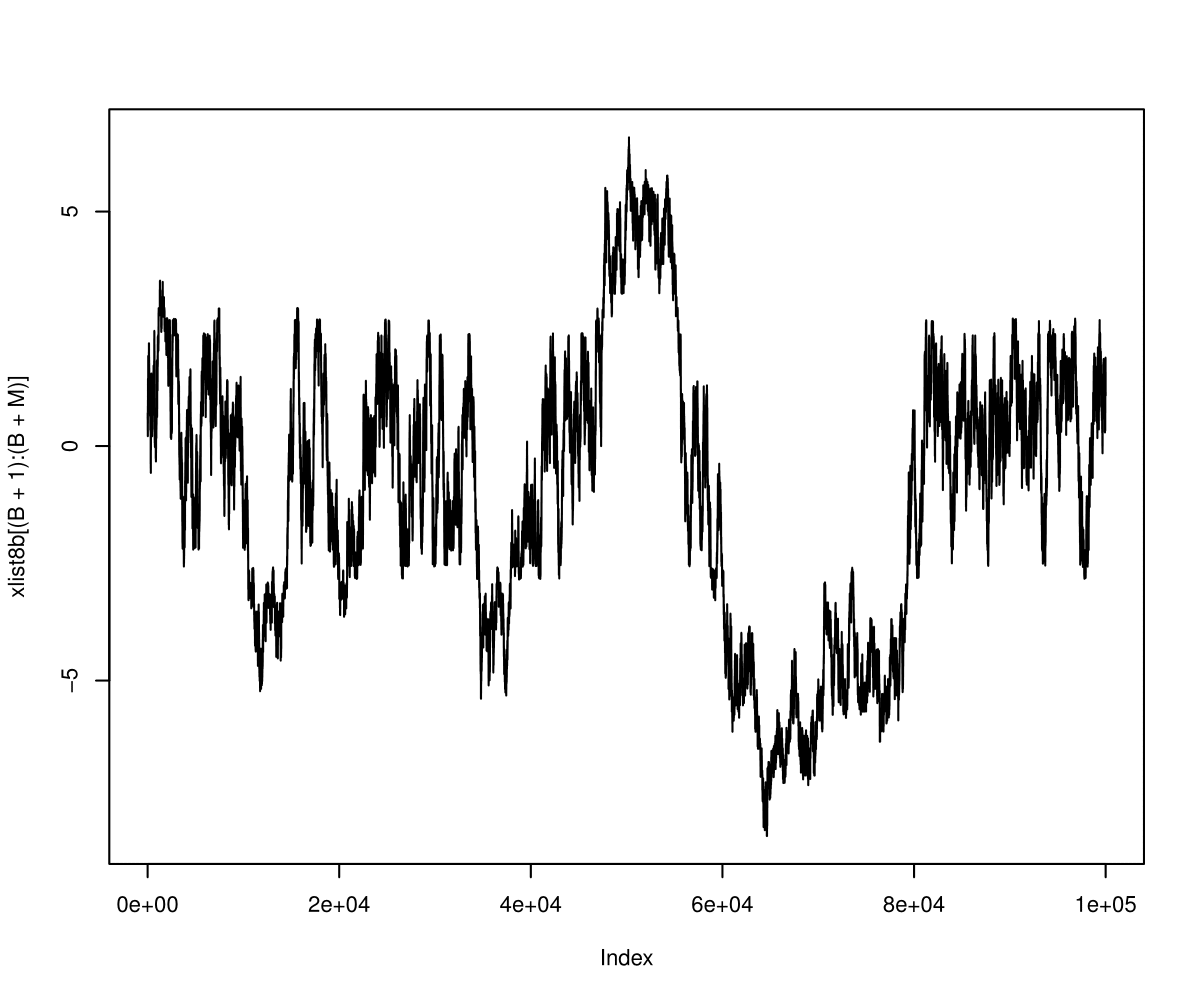
\includegraphics[width=\maxwidth]{figure/p8bplot-1} 

\end{knitrout}
		\caption{$x$ values of Langevin algorithm after burning-in}
\end{figure}

Notice that the estimation is by no means consistent, and the varfact values are huge, making the standar error large too.\\
\\
(c) Compare the two algorithms and discuss which one is "better".\\
In this case, the random-walk Metropolis algorithm clearly outperforms the Langevin algorithm as it produces more reasonable estimates to the integral. The Langevin algorithm is designed to work well for well behaved functions. In particular, if the function $g'(x)/g(x)$ is smooth, then the Langevin algorithm is going to outperform RWM algorithm. However, if we plot $g'(x)/g(x)$, we notice that it varies significantly even on a log-scaled plot
\begin{figure}[H]
  \centering
\begin{knitrout}
\definecolor{shadecolor}{rgb}{0.969, 0.969, 0.969}\color{fgcolor}\begin{kframe}
\begin{alltt}
\hlstd{xline} \hlkwb{=} \hlkwd{seq}\hlstd{(}\hlopt{-}\hlnum{10}\hlstd{,}\hlnum{10}\hlstd{,}\hlnum{0.01}\hlstd{)}
\hlkwd{plot}\hlstd{(}\hlkwd{log}\hlstd{(}\hlkwd{gp}\hlstd{(xline)}\hlopt{/}\hlkwd{g}\hlstd{(xline)),}\hlkwc{type}\hlstd{=}\hlstr{'l'}\hlstd{)}
\end{alltt}


{\ttfamily\noindent\color{warningcolor}{\#\# Warning in if (x >= 0) -exp(-x/10)/10 * (1 + cos(x) * sin(x\textasciicircum{}3)) + exp(-x/10) * : the condition has length > 1 and only the first element will be used}}

{\ttfamily\noindent\color{warningcolor}{\#\# Warning in log(gp(xline)/g(xline)): NaNs produced}}\end{kframe}
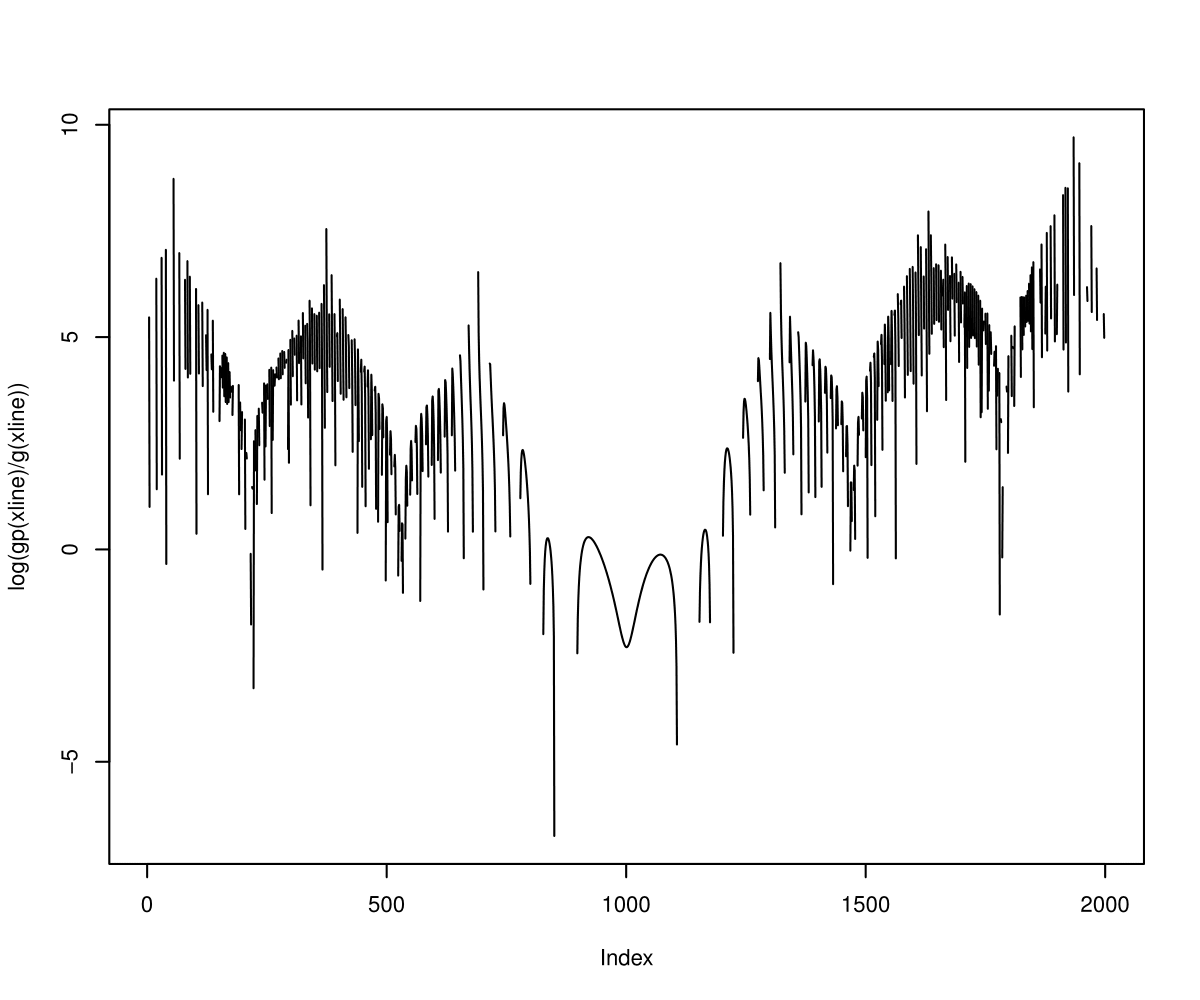
\includegraphics[width=\maxwidth]{figure/p8cplot-1} 

\end{knitrout}
\end{figure}
Since to the function $g'(x)/g(x)$ is unstable, a discrete approximation of this function will fail. As a result, the RWM algorithm outperforms the Langevin algorithm significantly.

\end{homeworkProblem}

\begin{homeworkProblem}

Consider the standard variance component model described in lecture, with $K=6$, $J_i=5$ and $\{Y_{ij}\}$ the famous "dyestuff" date, with prior values $a_1=a_2=a_3=b_1=b_2=b_3=100$. Estimate the posterior mean of $W/V$, in each of the three ways:\\
(a) With a random-walk Metropolis algorithm.
Since we are dealing with likelihood functions, we need to compute things in log-scale. The ratio of distributions becomes $$\log\left(\frac{g(Y)}{g(X)}\right) = \log g(Y)-\log g(X)$$
The initial $\theta_i$ values are reasonably assumed to follow a normal distribution centered at sample mean of $Y_{ij}$ with $V,W$ equal to the sample variance of $Y_{ij}$. \\
The RWM algorithm is implemented as follows:
\begin{knitrout}
\definecolor{shadecolor}{rgb}{0.969, 0.969, 0.969}\color{fgcolor}\begin{kframe}
\begin{alltt}
\hlstd{a}\hlkwb{=}\hlnum{100}
\hlstd{K}\hlkwb{=}\hlnum{6}
\hlstd{J}\hlkwb{=}\hlnum{5}

\hlstd{B}\hlkwb{=}\hlnum{2e+6}
\hlstd{M}\hlkwb{=}\hlnum{5e+5}
\hlstd{sigma} \hlkwb{=} \hlnum{7}

\hlstd{Ydye} \hlkwb{=} \hlkwd{t}\hlstd{(} \hlkwd{matrix}\hlstd{(}
  \hlkwd{c}\hlstd{(}\hlnum{1545}\hlstd{,} \hlnum{1440}\hlstd{,} \hlnum{1440}\hlstd{,} \hlnum{1520}\hlstd{,} \hlnum{1580}\hlstd{,}
    \hlnum{1540}\hlstd{,} \hlnum{1555}\hlstd{,} \hlnum{1490}\hlstd{,} \hlnum{1560}\hlstd{,} \hlnum{1495}\hlstd{,}
    \hlnum{1595}\hlstd{,} \hlnum{1550}\hlstd{,} \hlnum{1605}\hlstd{,} \hlnum{1510}\hlstd{,} \hlnum{1560}\hlstd{,}
    \hlnum{1445}\hlstd{,} \hlnum{1440}\hlstd{,} \hlnum{1595}\hlstd{,} \hlnum{1465}\hlstd{,} \hlnum{1545}\hlstd{,}
    \hlnum{1595}\hlstd{,} \hlnum{1630}\hlstd{,} \hlnum{1515}\hlstd{,} \hlnum{1635}\hlstd{,} \hlnum{1625}\hlstd{,}
    \hlnum{1520}\hlstd{,} \hlnum{1455}\hlstd{,} \hlnum{1450}\hlstd{,} \hlnum{1480}\hlstd{,} \hlnum{1445}\hlstd{),} \hlkwc{nrow}\hlstd{=}\hlnum{5}\hlstd{) )}

\hlstd{logg} \hlkwb{=} \hlkwa{function}\hlstd{(}\hlkwc{m}\hlstd{,}\hlkwc{V}\hlstd{,}\hlkwc{W}\hlstd{,}\hlkwc{theta}\hlstd{,}\hlkwc{Ydye}\hlstd{) \{}
  \hlstd{g} \hlkwb{=} \hlopt{-}\hlstd{a}\hlopt{/}\hlstd{V} \hlopt{+} \hlkwd{log}\hlstd{(}\hlkwd{max}\hlstd{(}\hlkwd{c}\hlstd{(V,}\hlnum{1e-5}\hlstd{)))}\hlopt{*}\hlstd{(}\hlopt{-}\hlstd{a}\hlopt{-}\hlnum{1}\hlstd{)} \hlopt{+} \hlstd{(}\hlopt{-}\hlstd{a}\hlopt{/}\hlstd{W)}
  \hlstd{g} \hlkwb{=} \hlstd{g} \hlopt{+} \hlkwd{log}\hlstd{(}\hlkwd{max}\hlstd{(}\hlkwd{c}\hlstd{(W,}\hlnum{1e-5}\hlstd{)))}\hlopt{*}\hlstd{(}\hlopt{-}\hlstd{a}\hlopt{-}\hlnum{1}\hlstd{)} \hlopt{-} \hlstd{(m}\hlopt{-}\hlstd{a)}\hlopt{^}\hlnum{2}\hlopt{/}\hlstd{a}\hlopt{/}\hlnum{2}
  \hlstd{g} \hlkwb{=} \hlstd{g} \hlopt{+} \hlkwd{log}\hlstd{(}\hlkwd{max}\hlstd{(}\hlkwd{c}\hlstd{(V,}\hlnum{1e-5}\hlstd{)))}\hlopt{*}\hlstd{(}\hlopt{-}\hlstd{K}\hlopt{/}\hlnum{2}\hlstd{)} \hlopt{+} \hlkwd{log}\hlstd{(}\hlkwd{max}\hlstd{(}\hlkwd{c}\hlstd{(W,}\hlnum{1e-5}\hlstd{)))}\hlopt{*}\hlstd{(}\hlopt{-}\hlstd{K}\hlopt{*}\hlstd{J}\hlopt{/}\hlnum{2}\hlstd{)}
  \hlstd{g} \hlkwb{=} \hlstd{g} \hlopt{-} \hlkwd{sum}\hlstd{((theta}\hlopt{-}\hlstd{m)}\hlopt{^}\hlnum{2}\hlstd{)}\hlopt{/}\hlstd{V}\hlopt{/}\hlnum{2} \hlopt{-} \hlkwd{sum}\hlstd{((Ydye}\hlopt{-}\hlstd{theta)}\hlopt{^}\hlnum{2}\hlstd{)}\hlopt{/}\hlstd{W}\hlopt{/}\hlnum{2}
  \hlkwd{return} \hlstd{(g)}
\hlstd{\}}

\hlstd{m} \hlkwb{=} \hlkwd{rnorm}\hlstd{(}\hlnum{1}\hlstd{,a,a)}
\hlstd{V} \hlkwb{=} \hlkwd{var}\hlstd{(}\hlkwd{c}\hlstd{(Ydye))}
\hlstd{W} \hlkwb{=} \hlkwd{var}\hlstd{(}\hlkwd{c}\hlstd{(Ydye))}
\hlstd{theta} \hlkwb{=} \hlkwd{rnorm}\hlstd{(K,}\hlkwd{mean}\hlstd{(Ydye),}\hlkwd{sqrt}\hlstd{(V))}
\hlstd{acc} \hlkwb{=} \hlnum{0}
\hlstd{fnlist} \hlkwb{=} \hlkwd{numeric}\hlstd{(B}\hlopt{+}\hlstd{M)}

\hlkwa{for} \hlstd{(i} \hlkwa{in} \hlnum{1}\hlopt{:}\hlstd{(B}\hlopt{+}\hlstd{M)) \{}
  \hlstd{eps_m} \hlkwb{=} \hlkwd{rnorm}\hlstd{(}\hlnum{1}\hlstd{,}\hlnum{0}\hlstd{,sigma)}
  \hlstd{eps_V} \hlkwb{=} \hlkwd{rnorm}\hlstd{(}\hlnum{1}\hlstd{,}\hlnum{0}\hlstd{,sigma)}
  \hlstd{eps_W} \hlkwb{=} \hlkwd{rnorm}\hlstd{(}\hlnum{1}\hlstd{,}\hlnum{0}\hlstd{,sigma)}
  \hlstd{eps_theta} \hlkwb{=} \hlkwd{rnorm}\hlstd{(K,}\hlnum{0}\hlstd{,sigma)}

  \hlstd{dg} \hlkwb{=} \hlkwd{logg}\hlstd{(m}\hlopt{+}\hlstd{eps_m,V}\hlopt{+}\hlstd{eps_V,W}\hlopt{+}\hlstd{eps_W,theta}\hlopt{+}\hlstd{eps_theta,Ydye)} \hlopt{-}
    \hlkwd{logg}\hlstd{(m,V,W,theta,Ydye)}
  \hlkwa{if} \hlstd{(}\hlkwd{runif}\hlstd{(}\hlnum{1}\hlstd{)}\hlopt{<=}\hlkwd{exp}\hlstd{(dg)) \{}
    \hlkwa{if} \hlstd{(i}\hlopt{>}\hlstd{B)}
      \hlstd{acc} \hlkwb{=} \hlstd{acc} \hlopt{+} \hlnum{1}
    \hlstd{m} \hlkwb{=} \hlstd{m}\hlopt{+}\hlstd{eps_m}
    \hlstd{V} \hlkwb{=} \hlstd{V}\hlopt{+}\hlstd{eps_V}
    \hlstd{W} \hlkwb{=} \hlstd{W}\hlopt{+}\hlstd{eps_W}
    \hlstd{theta} \hlkwb{=} \hlstd{theta}\hlopt{+}\hlstd{eps_theta}
  \hlstd{\}}
  \hlstd{fnlist[i]} \hlkwb{=} \hlstd{W}\hlopt{/}\hlstd{V}
\hlstd{\}}
\hlstd{funcmean} \hlkwb{=} \hlkwd{mean}\hlstd{(fnlist[(B}\hlopt{+}\hlnum{1}\hlstd{)}\hlopt{:}\hlstd{(M}\hlopt{+}\hlstd{B)])}
\hlstd{funciidse} \hlkwb{=} \hlkwd{sd}\hlstd{(fnlist[(B}\hlopt{+}\hlnum{1}\hlstd{)}\hlopt{:}\hlstd{(M}\hlopt{+}\hlstd{B)])}\hlopt{/}\hlkwd{sqrt}\hlstd{(M)}
\hlstd{acf_k} \hlkwb{=} \hlkwd{acf}\hlstd{(fnlist[(B}\hlopt{+}\hlnum{1}\hlstd{)}\hlopt{:}\hlstd{(M}\hlopt{+}\hlstd{B)],}\hlkwc{lag.max} \hlstd{=} \hlnum{1000}\hlstd{,}\hlkwc{plot} \hlstd{=} \hlnum{FALSE}\hlstd{)}\hlopt{$}\hlstd{acf}
\hlstd{varfact} \hlkwb{=} \hlnum{2}\hlopt{*}\hlkwd{sum}\hlstd{(acf_k)}\hlopt{-}\hlnum{1}
\hlstd{funcse} \hlkwb{=} \hlstd{funciidse}\hlopt{*}\hlkwd{sqrt}\hlstd{(varfact)}
\hlstd{accrate} \hlkwb{=} \hlstd{acc}\hlopt{/}\hlstd{M}

\hlkwd{cat}\hlstd{(}\hlstr{'B = '}\hlstd{,B,}\hlstr{', M = '}\hlstd{,M,}\hlstr{'\textbackslash{}n'}\hlstd{)}
\hlkwd{cat}\hlstd{(}\hlstr{'Number of samples accepted = '}\hlstd{,acc,}\hlstr{', acceptance rate = '}\hlstd{,accrate,}\hlstr{'\textbackslash{}n'}\hlstd{)}
\hlkwd{cat}\hlstd{(}\hlstr{'Estimate = '}\hlstd{,funcmean,}\hlstr{'\textbackslash{}n'}\hlstd{)}
\hlkwd{cat}\hlstd{(}\hlstr{'i.i.d. standard error = '}\hlstd{,funciidse,}\hlstr{'\textbackslash{}n'}\hlstd{)}
\hlkwd{cat}\hlstd{(}\hlstr{'varfact = '}\hlstd{,varfact,}\hlstr{'\textbackslash{}n'}\hlstd{)}
\hlkwd{cat}\hlstd{(}\hlstr{'Standard error = '}\hlstd{,funcse,}\hlstr{'\textbackslash{}n'}\hlstd{)}
\end{alltt}
\end{kframe}
\end{knitrout}
Output of several runs:
\begin{knitrout}
\definecolor{shadecolor}{rgb}{0.969, 0.969, 0.969}\color{fgcolor}\begin{kframe}
\begin{verbatim}
## B =  2e+06 , M =  5e+05 
## Number of samples accepted =  127952 , acceptance rate =  0.255904 
## Estimate =  0.006394276 
## i.i.d. standard error =  8.691605e-07 
## varfact =  222.6512 
## Standard error =  1.296918e-05
## B =  2e+06 , M =  5e+05 
## Number of samples accepted =  127690 , acceptance rate =  0.25538 
## Estimate =  0.005920185 
## i.i.d. standard error =  8.150501e-07 
## varfact =  259.4071 
## Standard error =  1.312729e-05
## B =  2e+06 , M =  5e+05 
## Number of samples accepted =  127896 , acceptance rate =  0.255792 
## Estimate =  0.006361079 
## i.i.d. standard error =  8.695236e-07 
## varfact =  242.357 
## Standard error =  1.353659e-05
## B =  2e+06 , M =  5e+05 
## Number of samples accepted =  127489 , acceptance rate =  0.254978 
## Estimate =  0.006515764 
## i.i.d. standard error =  9.252959e-07 
## varfact =  382.6875 
## Standard error =  1.810101e-05
## B =  2e+06 , M =  5e+05 
## Number of samples accepted =  128078 , acceptance rate =  0.256156 
## Estimate =  0.005825482 
## i.i.d. standard error =  8.563688e-07 
## varfact =  477.4472 
## Standard error =  1.871214e-05
\end{verbatim}
\end{kframe}
\end{knitrout}
The tabulated result is as follows:\\
\begin{center}
\begin{knitrout}
\definecolor{shadecolor}{rgb}{0.969, 0.969, 0.969}\color{fgcolor}
\begin{tabular}{r|r|r|r|r}
\hline
estimation & acc\_rate & seiid & varfact\_r & standard\_error\\
\hline
0.0063943 & 0.255904 & 9e-07 & 222.6512 & 1.30e-05\\
\hline
0.0059202 & 0.255380 & 8e-07 & 259.4071 & 1.31e-05\\
\hline
0.0063611 & 0.255792 & 9e-07 & 242.3570 & 1.35e-05\\
\hline
0.0065158 & 0.254978 & 9e-07 & 382.6875 & 1.81e-05\\
\hline
0.0058255 & 0.256156 & 9e-07 & 477.4472 & 1.87e-05\\
\hline
\end{tabular}


\end{knitrout}
\end{center}

\begin{figure}[H]
  \centering
\begin{knitrout}
\definecolor{shadecolor}{rgb}{0.969, 0.969, 0.969}\color{fgcolor}\begin{kframe}
\begin{alltt}
\hlkwd{plot}\hlstd{(fnlist[(B}\hlopt{+}\hlnum{1}\hlstd{)}\hlopt{:}\hlstd{(B}\hlopt{+}\hlstd{M)],}\hlkwc{type}\hlstd{=}\hlstr{'l'}\hlstd{)}
\end{alltt}
\end{kframe}
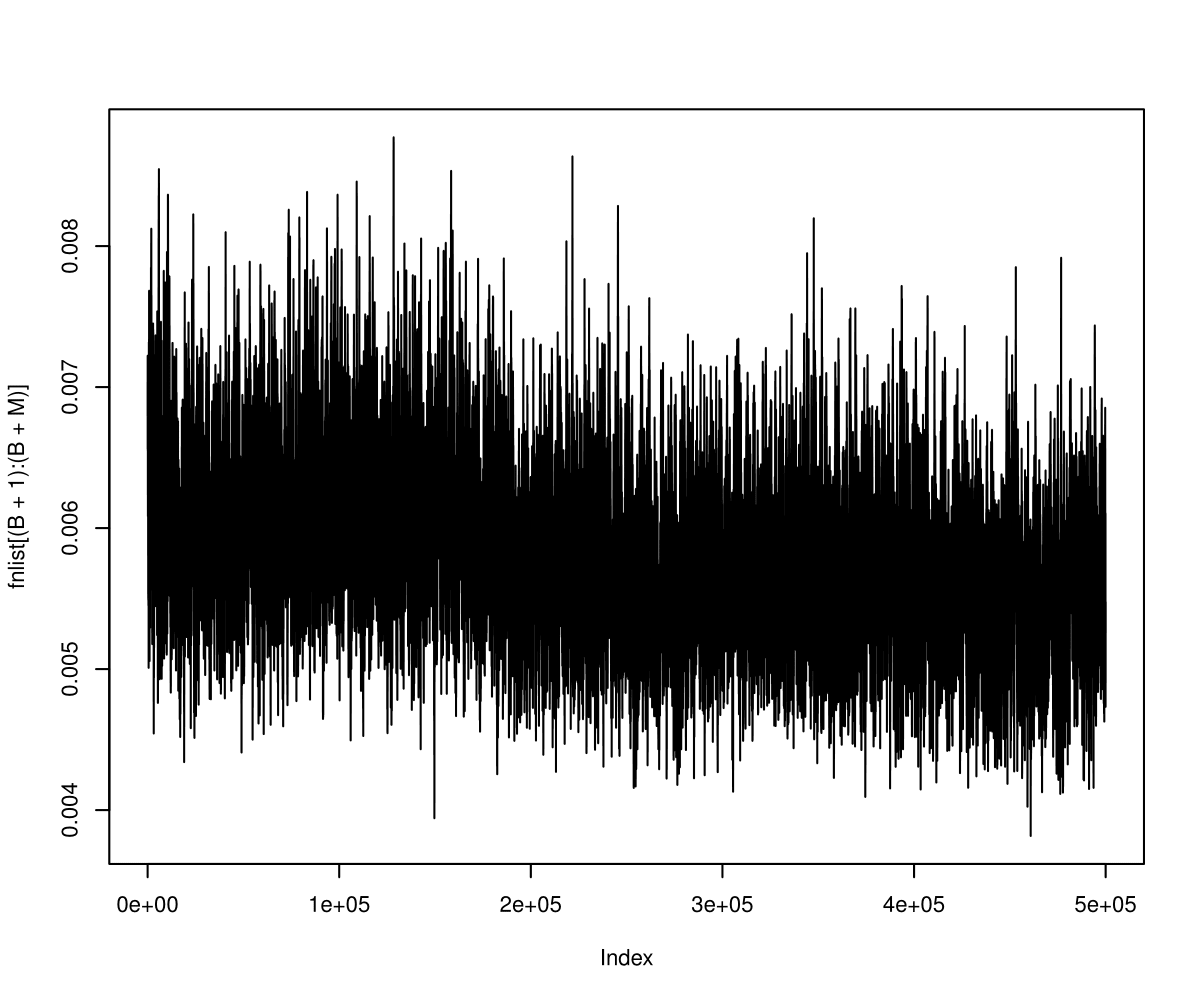
\includegraphics[width=\maxwidth]{figure/p9aplot-1} 

\end{knitrout}
		\caption{function values of Random-Walk Metropolis algorithm after burning-in}
\end{figure}
(b) With a Metropolis-within-Gibbs algorithm.
Using a Metropolis-within-Gibbs algorithem, we can safely increase $\sigma$. Source code:

\begin{knitrout}
\definecolor{shadecolor}{rgb}{0.969, 0.969, 0.969}\color{fgcolor}\begin{kframe}
\begin{alltt}
\hlstd{a}\hlkwb{=}\hlnum{100}
\hlstd{K}\hlkwb{=}\hlnum{6}
\hlstd{J}\hlkwb{=}\hlnum{5}

\hlstd{B}\hlkwb{=}\hlnum{1e+6}
\hlstd{M}\hlkwb{=}\hlnum{5e+5}
\hlstd{sigma} \hlkwb{=} \hlnum{40}

\hlstd{Ydye} \hlkwb{=} \hlkwd{t}\hlstd{(} \hlkwd{matrix}\hlstd{(}
  \hlkwd{c}\hlstd{(}\hlnum{1545}\hlstd{,} \hlnum{1440}\hlstd{,} \hlnum{1440}\hlstd{,} \hlnum{1520}\hlstd{,} \hlnum{1580}\hlstd{,}
    \hlnum{1540}\hlstd{,} \hlnum{1555}\hlstd{,} \hlnum{1490}\hlstd{,} \hlnum{1560}\hlstd{,} \hlnum{1495}\hlstd{,}
    \hlnum{1595}\hlstd{,} \hlnum{1550}\hlstd{,} \hlnum{1605}\hlstd{,} \hlnum{1510}\hlstd{,} \hlnum{1560}\hlstd{,}
    \hlnum{1445}\hlstd{,} \hlnum{1440}\hlstd{,} \hlnum{1595}\hlstd{,} \hlnum{1465}\hlstd{,} \hlnum{1545}\hlstd{,}
    \hlnum{1595}\hlstd{,} \hlnum{1630}\hlstd{,} \hlnum{1515}\hlstd{,} \hlnum{1635}\hlstd{,} \hlnum{1625}\hlstd{,}
    \hlnum{1520}\hlstd{,} \hlnum{1455}\hlstd{,} \hlnum{1450}\hlstd{,} \hlnum{1480}\hlstd{,} \hlnum{1445}\hlstd{),} \hlkwc{nrow}\hlstd{=}\hlnum{5}\hlstd{) )}

\hlstd{logg} \hlkwb{=} \hlkwa{function}\hlstd{(}\hlkwc{m}\hlstd{,}\hlkwc{V}\hlstd{,}\hlkwc{W}\hlstd{,}\hlkwc{theta}\hlstd{,}\hlkwc{Ydye}\hlstd{) \{}
  \hlstd{g} \hlkwb{=} \hlopt{-}\hlstd{a}\hlopt{/}\hlstd{V} \hlopt{+} \hlkwd{log}\hlstd{(}\hlkwd{max}\hlstd{(}\hlkwd{c}\hlstd{(V,}\hlnum{1e-5}\hlstd{)))}\hlopt{*}\hlstd{(}\hlopt{-}\hlstd{a}\hlopt{-}\hlnum{1}\hlstd{)} \hlopt{+} \hlstd{(}\hlopt{-}\hlstd{a}\hlopt{/}\hlstd{W)}
  \hlstd{g} \hlkwb{=} \hlstd{g} \hlopt{+} \hlkwd{log}\hlstd{(}\hlkwd{max}\hlstd{(}\hlkwd{c}\hlstd{(W,}\hlnum{1e-5}\hlstd{)))}\hlopt{*}\hlstd{(}\hlopt{-}\hlstd{a}\hlopt{-}\hlnum{1}\hlstd{)} \hlopt{-} \hlstd{(m}\hlopt{-}\hlstd{a)}\hlopt{^}\hlnum{2}\hlopt{/}\hlstd{a}\hlopt{/}\hlnum{2}
  \hlstd{g} \hlkwb{=} \hlstd{g} \hlopt{+} \hlkwd{log}\hlstd{(}\hlkwd{max}\hlstd{(}\hlkwd{c}\hlstd{(V,}\hlnum{1e-5}\hlstd{)))}\hlopt{*}\hlstd{(}\hlopt{-}\hlstd{K}\hlopt{/}\hlnum{2}\hlstd{)} \hlopt{+} \hlkwd{log}\hlstd{(}\hlkwd{max}\hlstd{(}\hlkwd{c}\hlstd{(W,}\hlnum{1e-5}\hlstd{)))}\hlopt{*}\hlstd{(}\hlopt{-}\hlstd{K}\hlopt{*}\hlstd{J}\hlopt{/}\hlnum{2}\hlstd{)}
  \hlstd{g} \hlkwb{=} \hlstd{g} \hlopt{-} \hlkwd{sum}\hlstd{((theta}\hlopt{-}\hlstd{m)}\hlopt{^}\hlnum{2}\hlstd{)}\hlopt{/}\hlstd{V}\hlopt{/}\hlnum{2} \hlopt{-} \hlkwd{sum}\hlstd{((Ydye}\hlopt{-}\hlstd{theta)}\hlopt{^}\hlnum{2}\hlstd{)}\hlopt{/}\hlstd{W}\hlopt{/}\hlnum{2}
  \hlkwd{return} \hlstd{(g)}
\hlstd{\}}

\hlstd{m} \hlkwb{=} \hlkwd{rnorm}\hlstd{(}\hlnum{1}\hlstd{,a,sigma)}
\hlstd{V} \hlkwb{=} \hlkwd{var}\hlstd{(}\hlkwd{c}\hlstd{(Ydye))}
\hlstd{W} \hlkwb{=} \hlkwd{var}\hlstd{(}\hlkwd{c}\hlstd{(Ydye))}
\hlstd{theta} \hlkwb{=} \hlkwd{rnorm}\hlstd{(K,}\hlkwd{mean}\hlstd{(Ydye),}\hlkwd{sqrt}\hlstd{(V))}
\hlstd{acc} \hlkwb{=} \hlnum{0}
\hlstd{fnlist} \hlkwb{=} \hlkwd{numeric}\hlstd{(B}\hlopt{+}\hlstd{M)}

\hlkwa{for} \hlstd{(i} \hlkwa{in} \hlnum{1}\hlopt{:}\hlstd{(B}\hlopt{+}\hlstd{M)) \{}
  \hlstd{eps_m}\hlkwb{=}\hlnum{0}
  \hlstd{eps_V}\hlkwb{=}\hlnum{0}
  \hlstd{eps_W}\hlkwb{=}\hlnum{0}
  \hlstd{eps_theta} \hlkwb{=} \hlkwd{rep}\hlstd{(}\hlnum{0}\hlstd{,K)}
  \hlstd{ci} \hlkwb{=} \hlstd{i} \hlopt \hlstd{(}\hlnum{3}\hlopt{+}\hlstd{K)}
  \hlkwa{if} \hlstd{(ci}\hlopt{==}\hlnum{0}\hlstd{)}
    \hlstd{eps_m} \hlkwb{=} \hlkwd{rnorm}\hlstd{(}\hlnum{1}\hlstd{,}\hlnum{0}\hlstd{,sigma)}
  \hlkwa{else if} \hlstd{(ci}\hlopt{==}\hlnum{1}\hlstd{)}
    \hlstd{eps_V} \hlkwb{=} \hlkwd{rnorm}\hlstd{(}\hlnum{1}\hlstd{,}\hlnum{0}\hlstd{,sigma)}
  \hlkwa{else if} \hlstd{(ci}\hlopt{==}\hlnum{2}\hlstd{)}
    \hlstd{eps_W} \hlkwb{=} \hlkwd{rnorm}\hlstd{(}\hlnum{1}\hlstd{,}\hlnum{0}\hlstd{,sigma)}
  \hlkwa{else}
    \hlstd{eps_theta[ci}\hlopt{-}\hlnum{2}\hlstd{]} \hlkwb{=} \hlkwd{rnorm}\hlstd{(}\hlnum{1}\hlstd{,}\hlnum{0}\hlstd{,sigma)}

  \hlstd{dg} \hlkwb{=} \hlkwd{logg}\hlstd{(m}\hlopt{+}\hlstd{eps_m,V}\hlopt{+}\hlstd{eps_V,W}\hlopt{+}\hlstd{eps_W,theta}\hlopt{+}\hlstd{eps_theta,Ydye)} \hlopt{-}
    \hlkwd{logg}\hlstd{(m,V,W,theta,Ydye)}
  \hlkwa{if} \hlstd{(}\hlkwd{runif}\hlstd{(}\hlnum{1}\hlstd{)}\hlopt{<=}\hlkwd{exp}\hlstd{(dg)) \{}
    \hlkwa{if} \hlstd{(i}\hlopt{>}\hlstd{B)}
    \hlstd{acc} \hlkwb{=} \hlstd{acc} \hlopt{+} \hlnum{1}
    \hlstd{m} \hlkwb{=} \hlstd{m}\hlopt{+}\hlstd{eps_m}
    \hlstd{V} \hlkwb{=} \hlstd{V}\hlopt{+}\hlstd{eps_V}
    \hlstd{W} \hlkwb{=} \hlstd{W}\hlopt{+}\hlstd{eps_W}
    \hlstd{theta} \hlkwb{=} \hlstd{theta}\hlopt{+}\hlstd{eps_theta}
  \hlstd{\}}
  \hlstd{fnlist[i]} \hlkwb{=} \hlstd{W}\hlopt{/}\hlstd{V}
\hlstd{\}}
\hlstd{funcmean} \hlkwb{=} \hlkwd{mean}\hlstd{(fnlist[(B}\hlopt{+}\hlnum{1}\hlstd{)}\hlopt{:}\hlstd{(M}\hlopt{+}\hlstd{B)])}
\hlstd{funciidse} \hlkwb{=} \hlkwd{sd}\hlstd{(fnlist[(B}\hlopt{+}\hlnum{1}\hlstd{)}\hlopt{:}\hlstd{(M}\hlopt{+}\hlstd{B)])}\hlopt{/}\hlkwd{sqrt}\hlstd{(M)}
\hlstd{acf_k} \hlkwb{=} \hlkwd{acf}\hlstd{(fnlist[(B}\hlopt{+}\hlnum{1}\hlstd{)}\hlopt{:}\hlstd{(M}\hlopt{+}\hlstd{B)],}\hlkwc{lag.max} \hlstd{=} \hlnum{1000}\hlstd{,}\hlkwc{plot} \hlstd{=} \hlnum{FALSE}\hlstd{)}\hlopt{$}\hlstd{acf}
\hlstd{varfact} \hlkwb{=} \hlnum{2}\hlopt{*}\hlkwd{sum}\hlstd{(acf_k)}\hlopt{-}\hlnum{1}
\hlstd{funcse} \hlkwb{=} \hlstd{funciidse}\hlopt{*}\hlkwd{sqrt}\hlstd{(varfact)}
\hlstd{accrate} \hlkwb{=} \hlstd{acc}\hlopt{/}\hlstd{M}

\hlkwd{cat}\hlstd{(}\hlstr{'B = '}\hlstd{,B,}\hlstr{', M = '}\hlstd{,M,}\hlstr{'\textbackslash{}n'}\hlstd{)}
\hlkwd{cat}\hlstd{(}\hlstr{'Number of samples accepted = '}\hlstd{,acc,}\hlstr{', acceptance rate = '}\hlstd{,accrate,}\hlstr{'\textbackslash{}n'}\hlstd{)}
\hlkwd{cat}\hlstd{(}\hlstr{'Estimate = '}\hlstd{,funcmean,}\hlstr{'\textbackslash{}n'}\hlstd{)}
\hlkwd{cat}\hlstd{(}\hlstr{'i.i.d. standard error = '}\hlstd{,funciidse,}\hlstr{'\textbackslash{}n'}\hlstd{)}
\hlkwd{cat}\hlstd{(}\hlstr{'varfact = '}\hlstd{,varfact,}\hlstr{'\textbackslash{}n'}\hlstd{)}
\hlkwd{cat}\hlstd{(}\hlstr{'Standard error = '}\hlstd{,funcse,}\hlstr{'\textbackslash{}n'}\hlstd{)}
\end{alltt}
\end{kframe}
\end{knitrout}
Output of several runs:
\begin{knitrout}
\definecolor{shadecolor}{rgb}{0.969, 0.969, 0.969}\color{fgcolor}\begin{kframe}
\begin{verbatim}
## B =  1e+06 , M =  5e+05 
## Number of samples accepted =  177717 , acceptance rate =  0.355434 
## Estimate =  0.005133218 
## i.i.d. standard error =  7.382176e-07 
## varfact =  298.7258 
## Standard error =  1.275912e-05
## B =  1e+06 , M =  5e+05 
## Number of samples accepted =  177155 , acceptance rate =  0.35431 
## Estimate =  0.004777328 
## i.i.d. standard error =  7.062485e-07 
## varfact =  357.6378 
## Standard error =  1.335609e-05
## B =  1e+06 , M =  5e+05 
## Number of samples accepted =  177056 , acceptance rate =  0.354112 
## Estimate =  0.004697013 
## i.i.d. standard error =  6.735418e-07 
## varfact =  305.6105 
## Standard error =  1.177467e-05
## B =  1e+06 , M =  5e+05 
## Number of samples accepted =  177643 , acceptance rate =  0.355286 
## Estimate =  0.004896768 
## i.i.d. standard error =  8.344297e-07 
## varfact =  779.2573 
## Standard error =  2.329326e-05
## B =  1e+06 , M =  5e+05 
## Number of samples accepted =  177505 , acceptance rate =  0.35501 
## Estimate =  0.004181851 
## i.i.d. standard error =  6.293576e-07 
## varfact =  411.9449 
## Standard error =  1.277371e-05
\end{verbatim}
\end{kframe}
\end{knitrout}
The tabulated result is as follows:\\
\begin{center}
\begin{knitrout}
\definecolor{shadecolor}{rgb}{0.969, 0.969, 0.969}\color{fgcolor}
\begin{tabular}{r|r|r|r|r}
\hline
estimation & acc\_rate & seiid & varfact\_r & standard\_error\\
\hline
0.0051332 & 0.355434 & 7e-07 & 298.7258 & 1.28e-05\\
\hline
0.0047773 & 0.354310 & 7e-07 & 357.6378 & 1.34e-05\\
\hline
0.0046970 & 0.354112 & 7e-07 & 305.6105 & 1.18e-05\\
\hline
0.0048968 & 0.355286 & 8e-07 & 779.2573 & 2.33e-05\\
\hline
0.0041819 & 0.355010 & 6e-07 & 411.9449 & 1.28e-05\\
\hline
\end{tabular}


\end{knitrout}
\end{center}
\begin{figure}[H]
  \centering
\begin{knitrout}
\definecolor{shadecolor}{rgb}{0.969, 0.969, 0.969}\color{fgcolor}\begin{kframe}
\begin{alltt}
\hlkwd{plot}\hlstd{(fnlist[(B}\hlopt{+}\hlnum{1}\hlstd{)}\hlopt{:}\hlstd{(B}\hlopt{+}\hlstd{M)],}\hlkwc{type}\hlstd{=}\hlstr{'l'}\hlstd{)}
\end{alltt}
\end{kframe}
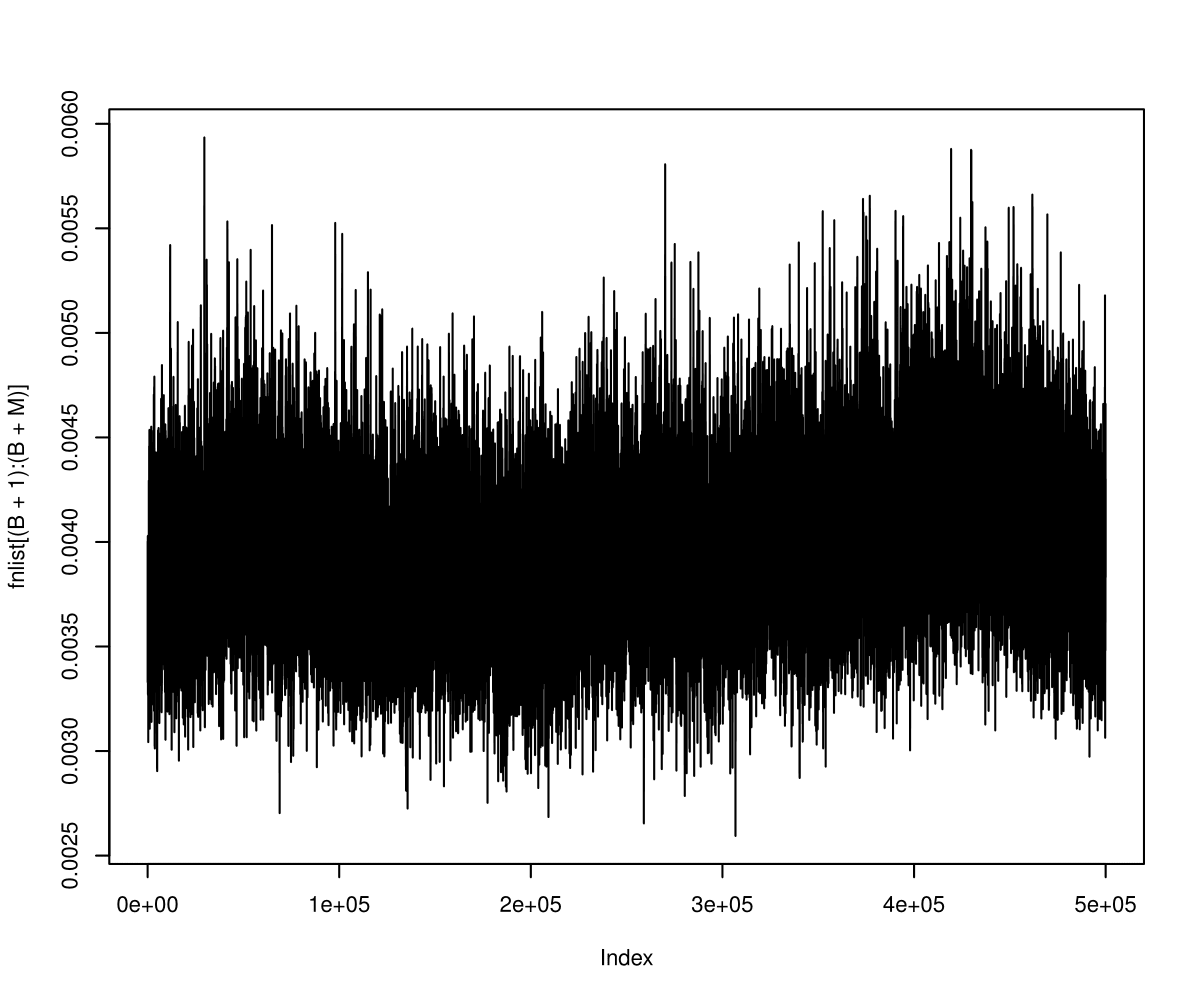
\includegraphics[width=\maxwidth]{figure/p9bplot-1} 

\end{knitrout}
		\caption{function values of Metropolis-within-Gibbs algorithm after burning-in}
\end{figure}
(c) With a Gibbs sampler.\\
For Gibbs sampler, we need to calculate the conditional distributions in closed form. \\
Firstly, the joint distribution is given by 
\begin{align*}
f(V,W,\mu,\theta,Y) = &Ce^{-b_1/V}V^{-a_1-1}e^{-b_2/W}W^{-a_2-1}e^{-(\mu-a3)^2/2b_3}V^{-K/2}W^{-\frac{1}{2}KJ}\times\\
                      &\exp\left[-\sum\limits_{i=1}^K(\theta_i-\mu)^2/2V - \sum\limits_{i=1}^K\sum\limits_{j=1}^J(Y_{ij}-\theta_i)^2/2W\right]\\
                       = &Ce^{-a/V}V^{-a-1}e^{-a/W}W^{-a-1}e^{-(\mu-a)^2/2a}V^{-K/2}W^{-\frac{1}{2}KJ}\times\\
                      &\exp\left[-\sum\limits_{i=1}^K(\theta_i-\mu)^2/2V - \sum\limits_{i=1}^K\sum\limits_{j=1}^J(Y_{ij}-\theta_i)^2/2W\right]
\end{align*}
where C is a normalizing constant, and $a=a_1=a_2=a_3=b_1=b_2=b_3$. \\
Now, we can write the following conditional distributions:
\begin{align*}
f(\mu|V,W,\theta) &= C\exp\left[-\frac{(\mu-a)^2}{2a}-\sum\limits_{i=1}^K\frac{(\theta_i-\mu)^2}{2V}\right]\\
    &= C\exp\left[-\mu^2\left(\frac{1}{2a}+\frac{K}{2V}\right)+\mu\left(1+\sum\limits_{i=1}^K\frac{\theta_i}{V}\right)\right]\\
\end{align*}
If we let $\mu|*$ to follow a $N(m,v)$ distribution for some $m$ and $v$, and match the coefficients to get
$$v=\left(\frac{1}{2a}+\frac{K}{2V}\right)^{-1}\bigg/2 = \left(\frac{1}{a}+\frac{K}{V}\right)^{-1}$$
$$m=\left(1+\sum\limits_{i=1}^K\frac{\theta_i}{V}\right)\left(\frac{1}{a}+\frac{K}{V}\right)^{-1}$$
Therefore, we have 
$$(\mu|V,W,\theta)\sim N\left(\left(1+\sum\limits_{i=1}^K\frac{\theta_i}{V}\right)\left(\frac{1}{a}+\frac{K}{V}\right)^{-1},\left(\frac{1}{a}+\frac{K}{V}\right)^{-1}\right)$$
\begin{align*}
f(V|\mu,W,\theta) &= Ce^{-a/V}V^{-a-1}V^{-K/2}\exp\left(-\sum\limits_{i=1}^K\frac{(\theta_i-\mu)^2}{2V}\right)\\
  &=CV^{-a-1-K/2}\exp\left(-\frac{1}{V}\left[a+\sum\limits_{i=1}^K\frac{(\theta_i-\mu)^2}{2}\right]\right)
\end{align*}
Notice that this is the pdf of a Inverse Gamma distribution with parameters $\alpha = a + K/2$ and $\beta = a+\sum_{i=1}^K(\theta_i-\mu)^2/2$, i.e. we have 
$$(V|\mu,W,\theta)\sim IG\left(a+\frac{K}{2}, a+\sum\limits_{i=1}^K\frac{(\theta_i-\mu)^2}{2}\right)$$
Similarly, 
\begin{align*}
f(W|\mu,V,\theta) &= Ce^{-a/W}W^{-a-1}W^{-KJ/2}\exp\left(-\frac{1}{W}\sum\limits_{i=1}^K\sum\limits_{j=1}^J\frac{(Y_{ij}-\theta_i)^2}{2}\right)\\
  &=CW^{-a-1-KJ/2}\exp\left(-\frac{1}{W}\left[a+\sum\limits_{i=1}^K\sum\limits_{j=1}^J\frac{(Y_{ij}-\theta_i)^2}{2}\right]\right)
  \end{align*}
Again, this is the pdf of Inverse Gamma distribution with parameters $\alpha = a+KJ/2$ and $\beta=a+\sum_{i=1}^K\sum_{j=1}^J(Y_{ij}-\theta_i)^2/2$. i.e.
$$(W|\mu,V,\theta)\sim IG\left(a+KJ/2,a+\sum\limits_{i=1}^K\sum\limits_{j=1}^J\frac{(Y_{ij}-\theta_i)^2}{2}\right)$$
Lastly, 
\begin{align*}
f(\theta_i|\mu,V,W) &= C\exp\left(-\frac{(\theta_i-\mu)^2}{2V}-\sum\limits_{j=1}^J\frac{(Y_{ij}-\theta_i)^2}{2W}\right)\\
  &=C\exp\left(-\theta_i^2\left(\frac{1}{2V}+\frac{J}{2W}\right)+\theta_i\left(\frac{\mu}{V}+\sum\limits_{j=1}^J\frac{Y_{ij}}{W}\right)\right)
\end{align*}
If we let $\mu|*$ to follow a $N(m,v)$ distribution for some $m$ and $v$, and match the coefficients to get
$$v = \left(\frac{1}{2V}+\frac{J}{2W}\right)^{-1}\bigg/ 2 = \left(\frac{1}{V}+\frac{J}{W}\right)^{-1}$$
$$m = \left(\frac{\mu}{V} + \sum\limits_{j=1}^J\frac{Y_{ij}}{W}\right)\left(\frac{1}{V}+\frac{J}{W}\right)^{-1}$$
i.e. we have 
$$(\theta_i|\mu,V,W)\sim N\left(\left(\frac{\mu}{V} + \sum\limits_{j=1}^J\frac{Y_{ij}}{W}\right)\left(\frac{1}{V}+\frac{J}{W}\right)^{-1},\left(\frac{1}{V}+\frac{J}{W}\right)^{-1}\right)$$
Finally, using the closed form conditional distribution above, we can implement the Gibbs sampler as follows:

\begin{knitrout}
\definecolor{shadecolor}{rgb}{0.969, 0.969, 0.969}\color{fgcolor}\begin{kframe}
\begin{alltt}
\hlstd{a}\hlkwb{=}\hlnum{100}
\hlstd{K}\hlkwb{=}\hlnum{6}
\hlstd{J}\hlkwb{=}\hlnum{5}

\hlstd{B}\hlkwb{=}\hlnum{1e+5}
\hlstd{M}\hlkwb{=}\hlnum{5e+5}
\hlstd{sigma} \hlkwb{=} \hlnum{20}

\hlstd{Ydye} \hlkwb{=} \hlkwd{t}\hlstd{(} \hlkwd{matrix}\hlstd{(}
  \hlkwd{c}\hlstd{(}\hlnum{1545}\hlstd{,} \hlnum{1440}\hlstd{,} \hlnum{1440}\hlstd{,} \hlnum{1520}\hlstd{,} \hlnum{1580}\hlstd{,}
    \hlnum{1540}\hlstd{,} \hlnum{1555}\hlstd{,} \hlnum{1490}\hlstd{,} \hlnum{1560}\hlstd{,} \hlnum{1495}\hlstd{,}
    \hlnum{1595}\hlstd{,} \hlnum{1550}\hlstd{,} \hlnum{1605}\hlstd{,} \hlnum{1510}\hlstd{,} \hlnum{1560}\hlstd{,}
    \hlnum{1445}\hlstd{,} \hlnum{1440}\hlstd{,} \hlnum{1595}\hlstd{,} \hlnum{1465}\hlstd{,} \hlnum{1545}\hlstd{,}
    \hlnum{1595}\hlstd{,} \hlnum{1630}\hlstd{,} \hlnum{1515}\hlstd{,} \hlnum{1635}\hlstd{,} \hlnum{1625}\hlstd{,}
    \hlnum{1520}\hlstd{,} \hlnum{1455}\hlstd{,} \hlnum{1450}\hlstd{,} \hlnum{1480}\hlstd{,} \hlnum{1445}\hlstd{),} \hlkwc{nrow}\hlstd{=}\hlnum{5}\hlstd{) )}

\hlstd{logg} \hlkwb{=} \hlkwa{function}\hlstd{(}\hlkwc{m}\hlstd{,}\hlkwc{V}\hlstd{,}\hlkwc{W}\hlstd{,}\hlkwc{theta}\hlstd{,}\hlkwc{Ydye}\hlstd{) \{}
  \hlstd{g} \hlkwb{=} \hlopt{-}\hlstd{a}\hlopt{/}\hlstd{V} \hlopt{+} \hlkwd{log}\hlstd{(}\hlkwd{max}\hlstd{(}\hlkwd{c}\hlstd{(V,}\hlnum{1e-5}\hlstd{)))}\hlopt{*}\hlstd{(}\hlopt{-}\hlstd{a}\hlopt{-}\hlnum{1}\hlstd{)} \hlopt{+} \hlstd{(}\hlopt{-}\hlstd{a}\hlopt{/}\hlstd{W)}
  \hlstd{g} \hlkwb{=} \hlstd{g} \hlopt{+} \hlkwd{log}\hlstd{(}\hlkwd{max}\hlstd{(}\hlkwd{c}\hlstd{(W,}\hlnum{1e-5}\hlstd{)))}\hlopt{*}\hlstd{(}\hlopt{-}\hlstd{a}\hlopt{-}\hlnum{1}\hlstd{)} \hlopt{-} \hlstd{(m}\hlopt{-}\hlstd{a)}\hlopt{^}\hlnum{2}\hlopt{/}\hlstd{a}\hlopt{/}\hlnum{2}
  \hlstd{g} \hlkwb{=} \hlstd{g} \hlopt{+} \hlkwd{log}\hlstd{(}\hlkwd{max}\hlstd{(}\hlkwd{c}\hlstd{(V,}\hlnum{1e-5}\hlstd{)))}\hlopt{*}\hlstd{(}\hlopt{-}\hlstd{K}\hlopt{/}\hlnum{2}\hlstd{)} \hlopt{+} \hlkwd{log}\hlstd{(}\hlkwd{max}\hlstd{(}\hlkwd{c}\hlstd{(W,}\hlnum{1e-5}\hlstd{)))}\hlopt{*}\hlstd{(}\hlopt{-}\hlstd{K}\hlopt{*}\hlstd{J}\hlopt{/}\hlnum{2}\hlstd{)}
  \hlstd{g} \hlkwb{=} \hlstd{g} \hlopt{-} \hlkwd{sum}\hlstd{((theta}\hlopt{-}\hlstd{m)}\hlopt{^}\hlnum{2}\hlstd{)}\hlopt{/}\hlstd{V}\hlopt{/}\hlnum{2} \hlopt{-} \hlkwd{sum}\hlstd{((Ydye}\hlopt{-}\hlstd{theta)}\hlopt{^}\hlnum{2}\hlstd{)}\hlopt{/}\hlstd{W}\hlopt{/}\hlnum{2}
  \hlkwd{return} \hlstd{(g)}
\hlstd{\}}

\hlstd{m} \hlkwb{=} \hlkwd{rnorm}\hlstd{(}\hlnum{1}\hlstd{,a,sigma)}
\hlstd{V} \hlkwb{=} \hlkwd{var}\hlstd{(}\hlkwd{c}\hlstd{(Ydye))}
\hlstd{W} \hlkwb{=} \hlkwd{var}\hlstd{(}\hlkwd{c}\hlstd{(Ydye))}
\hlstd{theta} \hlkwb{=} \hlkwd{rnorm}\hlstd{(K,}\hlkwd{mean}\hlstd{(Ydye),}\hlkwd{sqrt}\hlstd{(V))}
\hlstd{acc} \hlkwb{=} \hlnum{0}
\hlstd{fnlist} \hlkwb{=} \hlkwd{numeric}\hlstd{(B}\hlopt{+}\hlstd{M)}

\hlkwa{for} \hlstd{(i} \hlkwa{in} \hlnum{1}\hlopt{:}\hlstd{(B}\hlopt{+}\hlstd{M)) \{}
  \hlstd{eps_m}\hlkwb{=}\hlnum{0}
  \hlstd{eps_V}\hlkwb{=}\hlnum{0}
  \hlstd{eps_W}\hlkwb{=}\hlnum{0}
  \hlstd{eps_theta} \hlkwb{=} \hlkwd{rep}\hlstd{(}\hlnum{0}\hlstd{,K)}
  \hlstd{ci} \hlkwb{=} \hlstd{i} \hlopt \hlstd{(}\hlnum{3}\hlopt{+}\hlstd{K)}
  \hlkwa{if} \hlstd{(ci}\hlopt{==}\hlnum{0}\hlstd{)}
    \hlstd{m} \hlkwb{=} \hlkwd{rnorm}\hlstd{(}\hlnum{1}\hlstd{,}\hlnum{1}\hlopt{+}\hlkwd{sum}\hlstd{(theta)}\hlopt{/}\hlstd{V}\hlopt{/}\hlstd{(}\hlnum{1}\hlopt{/}\hlstd{a}\hlopt{+}\hlstd{K}\hlopt{/}\hlstd{V),(}\hlnum{1}\hlopt{/}\hlstd{a} \hlopt{+} \hlstd{K}\hlopt{/}\hlstd{V)}\hlopt{^}\hlstd{(}\hlopt{-}\hlnum{0.5}\hlstd{))}
  \hlkwa{else if} \hlstd{(ci}\hlopt{==}\hlnum{1}\hlstd{)}
    \hlstd{V} \hlkwb{=} \hlnum{1}\hlopt{/}\hlkwd{rgamma}\hlstd{(}\hlnum{1}\hlstd{,a}\hlopt{+}\hlstd{K}\hlopt{/}\hlnum{2}\hlstd{,a}\hlopt{+}\hlkwd{sum}\hlstd{((theta}\hlopt{-}\hlstd{m)}\hlopt{^}\hlnum{2}\hlstd{)}\hlopt{/}\hlnum{2}\hlstd{)}
  \hlkwa{else if} \hlstd{(ci}\hlopt{==}\hlnum{2}\hlstd{)}
    \hlstd{W} \hlkwb{=} \hlnum{1}\hlopt{/}\hlkwd{rgamma}\hlstd{(}\hlnum{1}\hlstd{,a}\hlopt{+}\hlstd{K}\hlopt{*}\hlstd{J}\hlopt{/}\hlnum{2}\hlstd{, a}\hlopt{+}\hlkwd{sum}\hlstd{((Ydye}\hlopt{-}\hlstd{theta)}\hlopt{^}\hlnum{2}\hlstd{)}\hlopt{/}\hlnum{2}\hlstd{)}
  \hlkwa{else}
    \hlstd{theta[ci}\hlopt{-}\hlnum{2}\hlstd{]} \hlkwb{=} \hlkwd{rnorm}\hlstd{(}\hlnum{1}\hlstd{,(m}\hlopt{/}\hlstd{V}\hlopt{+}\hlkwd{sum}\hlstd{(Ydye[ci}\hlopt{-}\hlnum{2}\hlstd{,])}\hlopt{/}\hlstd{W)}\hlopt{/}\hlstd{(}\hlnum{1}\hlopt{/}\hlstd{V}\hlopt{+}\hlstd{J}\hlopt{/}\hlstd{W),}
                        \hlstd{(}\hlnum{1}\hlopt{/}\hlstd{V}\hlopt{+}\hlstd{J}\hlopt{/}\hlstd{W)}\hlopt{^}\hlstd{(}\hlopt{-}\hlnum{0.5}\hlstd{))}

  \hlstd{fnlist[i]} \hlkwb{=} \hlstd{W}\hlopt{/}\hlstd{V}
\hlstd{\}}
\hlstd{funcmean} \hlkwb{=} \hlkwd{mean}\hlstd{(fnlist[(B}\hlopt{+}\hlnum{1}\hlstd{)}\hlopt{:}\hlstd{(M}\hlopt{+}\hlstd{B)])}
\hlstd{funciidse} \hlkwb{=} \hlkwd{sd}\hlstd{(fnlist[(B}\hlopt{+}\hlnum{1}\hlstd{)}\hlopt{:}\hlstd{(M}\hlopt{+}\hlstd{B)])}\hlopt{/}\hlkwd{sqrt}\hlstd{(M)}
\hlstd{acf_k} \hlkwb{=} \hlkwd{acf}\hlstd{(fnlist[(B}\hlopt{+}\hlnum{1}\hlstd{)}\hlopt{:}\hlstd{(M}\hlopt{+}\hlstd{B)],}\hlkwc{lag.max} \hlstd{=} \hlnum{1000}\hlstd{,}\hlkwc{plot} \hlstd{=} \hlnum{FALSE}\hlstd{)}\hlopt{$}\hlstd{acf}
\hlstd{varfact} \hlkwb{=} \hlnum{2}\hlopt{*}\hlkwd{sum}\hlstd{(acf_k)}\hlopt{-}\hlnum{1}
\hlstd{funcse} \hlkwb{=} \hlstd{funciidse}\hlopt{*}\hlkwd{sqrt}\hlstd{(varfact)}
\hlstd{accrate} \hlkwb{=} \hlstd{acc}\hlopt{/}\hlstd{M}

\hlkwd{cat}\hlstd{(}\hlstr{'B = '}\hlstd{,B,}\hlstr{', M = '}\hlstd{,M,}\hlstr{'\textbackslash{}n'}\hlstd{)}
\hlkwd{cat}\hlstd{(}\hlstr{'Number of samples accepted = '}\hlstd{,acc,}\hlstr{', acceptance rate = '}\hlstd{,accrate,}\hlstr{'\textbackslash{}n'}\hlstd{)}
\hlkwd{cat}\hlstd{(}\hlstr{'Estimate = '}\hlstd{,funcmean,}\hlstr{'\textbackslash{}n'}\hlstd{)}
\hlkwd{cat}\hlstd{(}\hlstr{'i.i.d. standard error = '}\hlstd{,funciidse,}\hlstr{'\textbackslash{}n'}\hlstd{)}
\hlkwd{cat}\hlstd{(}\hlstr{'varfact = '}\hlstd{,varfact,}\hlstr{'\textbackslash{}n'}\hlstd{)}
\hlkwd{cat}\hlstd{(}\hlstr{'Standard error = '}\hlstd{,funcse,}\hlstr{'\textbackslash{}n'}\hlstd{)}
\end{alltt}
\end{kframe}
\end{knitrout}
Output of several runs:
\begin{knitrout}
\definecolor{shadecolor}{rgb}{0.969, 0.969, 0.969}\color{fgcolor}\begin{kframe}
\begin{verbatim}
## B =  1e+05 , M =  5e+05 
## Number of samples accepted =  0 , acceptance rate =  0 
## Estimate =  0.003992738 
## i.i.d. standard error =  7.8035e-07 
## varfact =  11.25486 
## Standard error =  2.617939e-06
## B =  1e+05 , M =  5e+05 
## Number of samples accepted =  0 , acceptance rate =  0 
## Estimate =  0.00399849 
## i.i.d. standard error =  7.796216e-07 
## varfact =  10.92722 
## Standard error =  2.577144e-06
## B =  1e+05 , M =  5e+05 
## Number of samples accepted =  0 , acceptance rate =  0 
## Estimate =  0.003996011 
## i.i.d. standard error =  7.800165e-07 
## varfact =  8.801791 
## Standard error =  2.314138e-06
## B =  1e+05 , M =  5e+05 
## Number of samples accepted =  0 , acceptance rate =  0 
## Estimate =  0.003992633 
## i.i.d. standard error =  7.772488e-07 
## varfact =  10.07245 
## Standard error =  2.466764e-06
## B =  1e+05 , M =  5e+05 
## Number of samples accepted =  0 , acceptance rate =  0 
## Estimate =  0.003994966 
## i.i.d. standard error =  7.799505e-07 
## varfact =  10.16798 
## Standard error =  2.487049e-06
\end{verbatim}
\end{kframe}
\end{knitrout}
The tabulated result is as follows:\\
\begin{center}
\begin{knitrout}
\definecolor{shadecolor}{rgb}{0.969, 0.969, 0.969}\color{fgcolor}
\begin{tabular}{r|r|r|r}
\hline
estimation & seiid & varfact\_r & standard\_error\\
\hline
0.0039927 & 8e-07 & 11.254861 & 2.6e-06\\
\hline
0.0039985 & 8e-07 & 10.927216 & 2.6e-06\\
\hline
0.0039960 & 8e-07 & 8.801791 & 2.3e-06\\
\hline
0.0039926 & 8e-07 & 10.072450 & 2.5e-06\\
\hline
0.0039950 & 8e-07 & 10.167975 & 2.5e-06\\
\hline
\end{tabular}


\end{knitrout}
\end{center}
\begin{figure}[H]
  \centering
\begin{knitrout}
\definecolor{shadecolor}{rgb}{0.969, 0.969, 0.969}\color{fgcolor}\begin{kframe}
\begin{alltt}
\hlkwd{plot}\hlstd{(fnlist[(B}\hlopt{+}\hlnum{1}\hlstd{)}\hlopt{:}\hlstd{(B}\hlopt{+}\hlstd{M)],}\hlkwc{type}\hlstd{=}\hlstr{'l'}\hlstd{)}
\end{alltt}
\end{kframe}
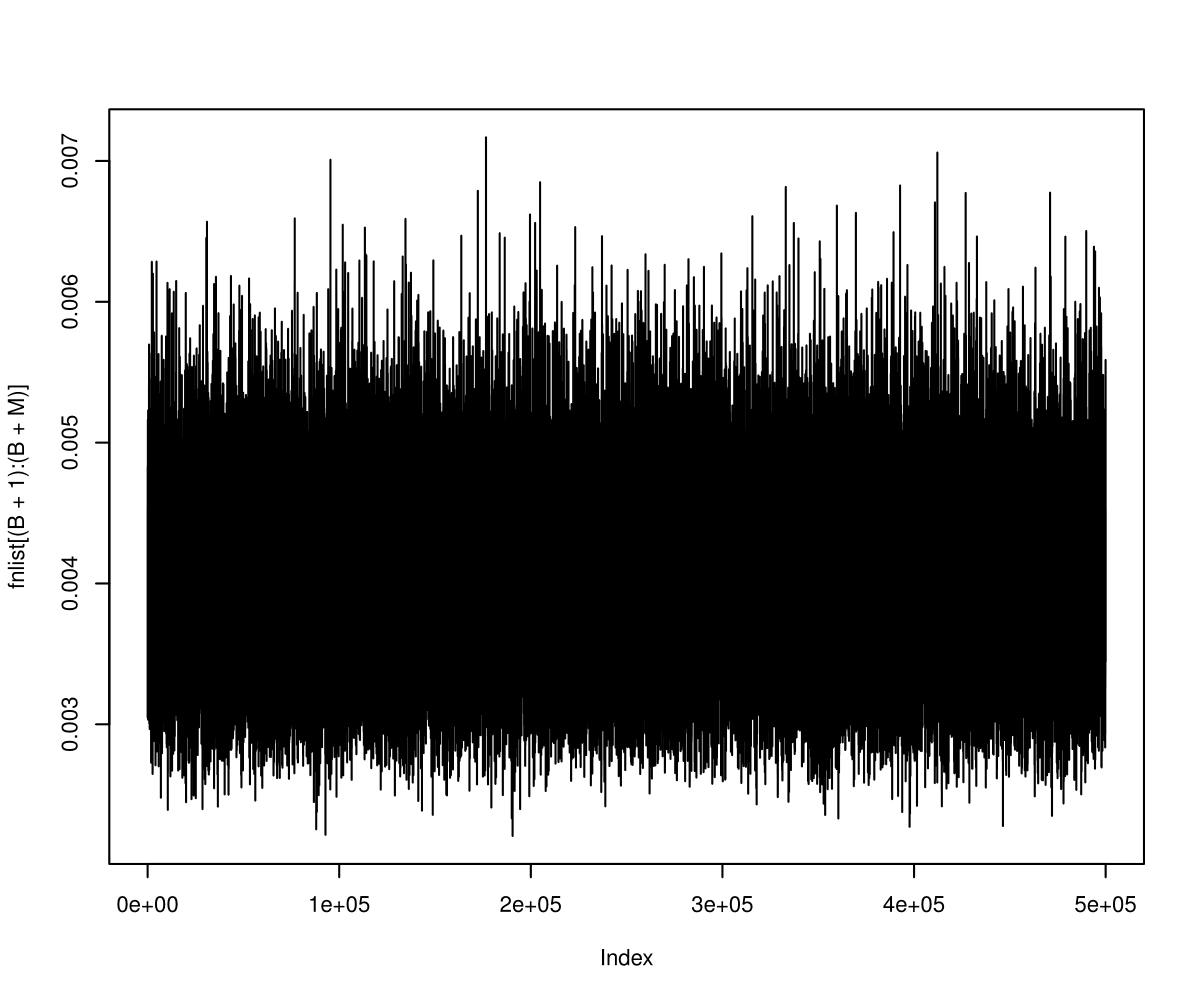
\includegraphics[width=\maxwidth]{figure/p9cplot-1} 

\end{knitrout}
		\caption{function values of Gibbs sampler after burning-in}
\end{figure}
(d) In terms of performance, the Gibbs sampler performs the best among the three as it requires the least amount of burning-in. The random-walk Metropolis requires 2e+6 steps just to burn-in to consistently generates non-trending function values (The function estimates tend to decrease over time if not burnt-in properly). This is quite a waste of computation power. The Metropolis-within-Gibbs requires similar number of steps to burn-in. On the contrary, the Gibbs sampler algorithm requires less than 1e+5 cycles to burn-in, which is magnitudes less than the required burning-in cycles for the other two algorithms. \\
The Gibbs sampler algorithm also performs better in terms of standard error since they produce low varfact values, meaning that the samples generated from the Gibbs sampler algorithm are close to i.i.d. samples. \\
However, the Gibbs sampler requires us to compute the conditional distribution in closed form, which may be very tedious and often impossible. The other two algorithms do not require analytic computation (choosing conjugate priors), hence they are much more easily implemented. \\
The Metropolis-within-Gibbs algorithm converges faster when comparing with the random-walk Metropolis algorithm. This is because the RWM proposes points that differs in all dimensions and will cause a higher chance of rejection.\\
Despite all these disadvantages, there are some advantages to the Random-Walk Metropolis algorithm. For example, if the distribution is defined on two regions that are disconnected in more than one dimension, then the Gibbs-like algorithms will not be able to travel from one region to the other. 

\end{homeworkProblem}

\begin{homeworkProblem}


\subsection{Term Structure of Interest Rates}
According to definition on INVESTOPEDIA, "the term structure of interest rates is the relationship between interest rates or bond yields and different terms or maturities. The term structure of interest rates is also known as a yield curve and it plays central role in an economy. The term structure reflects expectations of market participants about future changes in interest rates and their assessment of monetory policy conditions"\\
In mathematical finance, the term structure of interest rates is often modeled using stochastic methods, which can pose a number of difficult problems for estimation. One of the most crucial problems is that the parameters enter the state space in a highly nonlinear fasion. However, solving these non-linear systems are often quite rewarding as we can derive bonds and their derivatives prices from the models, yet, most of the time, we can only use MCMC methods to help solving the system.
\subsection{Vasicek's Model With Jumps}
The Vasicek's model assumes that the instantaneous spot rate is a Gaussian diffusion:
\begin{align*}
  dr_t &= \kappa_r(\theta_r-r_t)dt+\sigma_rdW_t^r\\
  dr_t &= (a_r+b_r r_t)dt+\sigma_rdW_t^r
\end{align*}
where $W_t^r$ is a Brownian motion under the objective measure, $P$, and we will work with the $(a_r,b_r)$ parameterization of the drift. \\
Baz and Das (1996) consider an extension of Vasicek's model to incorporate jumps in the short rate:
$$dr_t=(a_r-b_rr_{t-})dt +\sigma_r dW_t^r + d\left(\sum\limits_{j=1}^{N_t}\xi_{\tau_j}\right)$$
where we assume that $N_t$ is a Poisson process with constant intensity $\lambda$ and the jumps sizes are i.i.d. normal $\xi_{\tau_j}\sim N(\mu_J,\sigma_J^2)$. To value bonds under this model, we assume that the market price of interest rate risk is $\lambda_t=\lambda_r\sqrt{r_t}$  and if we assume the diffusive risk premium is constant, that $N_t^Q$ is a Poisson process under $Q$ with constant intensity $\lambda^Q$ and that the jump sizes are normally distributed under $Q$, $\xi_{\tau_j}^Q\sim N\left(\mu_j^Q,(\sigma_J^2)^Q\right)$, the evolution of the spot rate under $Q$ is then
$$dr_t = \kappa_r(\theta_r^Q-r_t)dt+\sigma_rdW_t^r(Q)+d\left(\sum\limits_{j=1}^{N_t^Q}\xi_{\tau_j}^Q\right)$$
where $W_t^r(Q)$ is a standard Brownian motion under the equivalent martingale measure $Q$. Then under this model, Using Feyman Kac's theorem, the price a non-defaultable zero coupon bond is given by
$$P(r_t,\tau)=E_t^Q\left[e^{-\int_t^{t+\tau}r_sds}\right]$$
\subsection{Monte Carlo Simulation and Integration Implementation}
In this mini-project, we assume the following parameter values 
\begin{align*}
  \tau &= 10\\
  \theta_r^Q &= 0.04\\
  r_t &= 0.015\\
  \kappa_r &= 0.6\\
  \sigma_r &= 0.03\\
  \lambda^Q &= 2\\
  \mu_J^Q &= 0\\
  (\sigma_J^2)^Q &= 0.01
\end{align*}
For small $h$, at any instance $t$, the distribution of $r_{t+h}$ given $r_t$ follows 
$$f(r_{t+h}|r_t) \sim N(r_t+\kappa_r(\theta_r^Q-r_t)h,(\sigma_r^2)^Q\sqrt{h}+Bernuolli(\lambda^Qh)*N\left(\mu_J^Q,(\sigma_J^2)^Q\right)$$
Using the distribution above, we simulate $M=2000$ paths and use Monte Carlo integration techiniques to calculate the price of zero-coupon bond. Ten runs are executed to investigate the consistency of the estimate.\\
Source code:\\
\begin{knitrout}
\definecolor{shadecolor}{rgb}{0.969, 0.969, 0.969}\color{fgcolor}\begin{kframe}
\begin{alltt}
\hlcom{#calculate the price of zero coupon bonds with Vasicek}
\hlcom{#with jump models}

\hlcom{#financial parameters (all adjusted for risk neutral measure)}
\hlstd{T} \hlkwb{=} \hlnum{10}
\hlstd{theta} \hlkwb{=} \hlnum{0.04}
\hlstd{cr} \hlkwb{=} \hlnum{0.015}
\hlstd{kappa} \hlkwb{=} \hlnum{0.6}
\hlstd{sigma} \hlkwb{=} \hlnum{0.03}
\hlstd{lambda} \hlkwb{=} \hlnum{2}
\hlstd{sigmaj} \hlkwb{=} \hlnum{0.01}
\hlstd{muj} \hlkwb{=} \hlnum{0}

\hlcom{#time interval set to be 0.01 to make 100 intervals per year}
\hlstd{h}\hlkwb{=}\hlnum{0.01}
\hlstd{M} \hlkwb{=} \hlnum{2000}
\hlstd{num} \hlkwb{=} \hlkwd{round}\hlstd{(T}\hlopt{/}\hlstd{h)}
\hlstd{vallist} \hlkwb{=} \hlkwd{rep}\hlstd{(}\hlnum{0}\hlstd{,M)}
\hlstd{plotX} \hlkwb{=} \hlkwd{matrix}\hlstd{(}\hlkwc{nrow} \hlstd{=} \hlnum{20}\hlstd{,} \hlkwc{ncol} \hlstd{= num}\hlopt{+}\hlnum{1}\hlstd{)}
\hlkwa{for} \hlstd{(j} \hlkwa{in} \hlnum{1}\hlopt{:}\hlstd{M) \{}
  \hlstd{X} \hlkwb{=} \hlkwd{rep}\hlstd{(}\hlnum{0}\hlstd{,num}\hlopt{+}\hlnum{1}\hlstd{)}
  \hlstd{X[}\hlnum{1}\hlstd{]} \hlkwb{=} \hlstd{cr}
  \hlkwa{for} \hlstd{(i} \hlkwa{in} \hlnum{1}\hlopt{:}\hlstd{num) \{}
    \hlkwa{if} \hlstd{(}\hlkwd{runif}\hlstd{(}\hlnum{1}\hlstd{)}\hlopt{<}\hlstd{lambda}\hlopt{*}\hlstd{h) \{jump} \hlkwb{=} \hlkwd{rnorm}\hlstd{(}\hlnum{1}\hlstd{,muj,sigmaj)\}}
    \hlkwa{else} \hlstd{jump} \hlkwb{=} \hlnum{0}
    \hlstd{X[i}\hlopt{+}\hlnum{1}\hlstd{]} \hlkwb{=} \hlkwd{rnorm}\hlstd{(}\hlnum{1}\hlstd{,X[i]}\hlopt{+}\hlstd{kappa}\hlopt{*}\hlstd{(theta}\hlopt{-}\hlstd{X[i])}\hlopt{*}\hlstd{h,sigma}\hlopt{*}\hlkwd{sqrt}\hlstd{(h))}\hlopt{+}\hlstd{jump}
    \hlkwa{if} \hlstd{(j}\hlopt{<=}\hlnum{20}\hlstd{) plotX[j,]} \hlkwb{=} \hlstd{X}
  \hlstd{\}}
  \hlstd{vallist[j]} \hlkwb{=} \hlkwd{exp}\hlstd{(}\hlopt{-}\hlkwd{sum}\hlstd{(X)}\hlopt{*}\hlstd{h)}
\hlstd{\}}
\hlstd{price} \hlkwb{=} \hlkwd{mean}\hlstd{(vallist)}
\hlstd{se} \hlkwb{=} \hlkwd{sd}\hlstd{(vallist)}\hlopt{/}\hlkwd{sqrt}\hlstd{(M)}
\hlkwd{cat}\hlstd{(}\hlstr{'The estimated zero-coupon bond price is '}\hlstd{,price,}\hlstr{'\textbackslash{}n'}\hlstd{)}
\hlkwd{cat}\hlstd{(}\hlstr{'The standard error is '}\hlstd{,se,}\hlstr{'\textbackslash{}n'}\hlstd{)}
\end{alltt}
\end{kframe}
\end{knitrout}
Output of several runs:
\begin{knitrout}
\definecolor{shadecolor}{rgb}{0.969, 0.969, 0.969}\color{fgcolor}\begin{kframe}
\begin{verbatim}
## The estimated zero-coupon bond price is  0.7043499 
## The standard error is  0.002424588
## The estimated zero-coupon bond price is  0.706554 
## The standard error is  0.002378813
## The estimated zero-coupon bond price is  0.7110355 
## The standard error is  0.002479945
## The estimated zero-coupon bond price is  0.7031318 
## The standard error is  0.002333143
## The estimated zero-coupon bond price is  0.7018515 
## The standard error is  0.002379074
## The estimated zero-coupon bond price is  0.7057709 
## The standard error is  0.002414406
## The estimated zero-coupon bond price is  0.7024047 
## The standard error is  0.002393151
## The estimated zero-coupon bond price is  0.7087772 
## The standard error is  0.002428283
## The estimated zero-coupon bond price is  0.7051398 
## The standard error is  0.002356732
## The estimated zero-coupon bond price is  0.7117877 
## The standard error is  0.00238904
\end{verbatim}
\end{kframe}
\end{knitrout}
The tabulated result is as follows:\\
\begin{center}
\begin{knitrout}
\definecolor{shadecolor}{rgb}{0.969, 0.969, 0.969}\color{fgcolor}
\begin{tabular}{r|r}
\hline
estprice & estse\\
\hline
0.7043499 & 0.0024246\\
\hline
0.7065540 & 0.0023788\\
\hline
0.7110355 & 0.0024799\\
\hline
0.7031318 & 0.0023331\\
\hline
0.7018515 & 0.0023791\\
\hline
0.7057709 & 0.0024144\\
\hline
0.7024047 & 0.0023932\\
\hline
0.7087772 & 0.0024283\\
\hline
0.7051398 & 0.0023567\\
\hline
0.7117877 & 0.0023890\\
\hline
\end{tabular}


\end{knitrout}
\end{center}
From the table above, we can see that the estimated price is fairly consistent with a mean of 0.7060803. The standard error of the price is also relatively small, the mean of the estimated standard error is 0.0023977. The standard error calculated from multiple runs of executing the program is 0.0034751. The small standar error of the estimated price means our MC estimation is reasonably accurate. \\
There are several advantages to this approach.\\
First of all, since there are multiple sources of stochasticity in our model (namely, the diffusive brownian motion, the number of jumps and the size jumps), solving the system analytically is (almost) impossible. In order to find a reasonable bond price under this model, we have to use MC simulation method.\\
Also, since we have simulated paths of realizations of the spot rate, we can also find out how risky the bond is. That is, if we invest the same amount in the bank account and follow the simulated spot rate paths, how much more or less we are going to make in comparison to investing in the zero-coupon bond. \\
Last but not least, we can look at some sample paths of the spot rate curve to see if our model assumption is valid. The following figure outlines 20 sample paths from our simulation
\begin{figure}[H]
  \centering
\begin{knitrout}
\definecolor{shadecolor}{rgb}{0.969, 0.969, 0.969}\color{fgcolor}
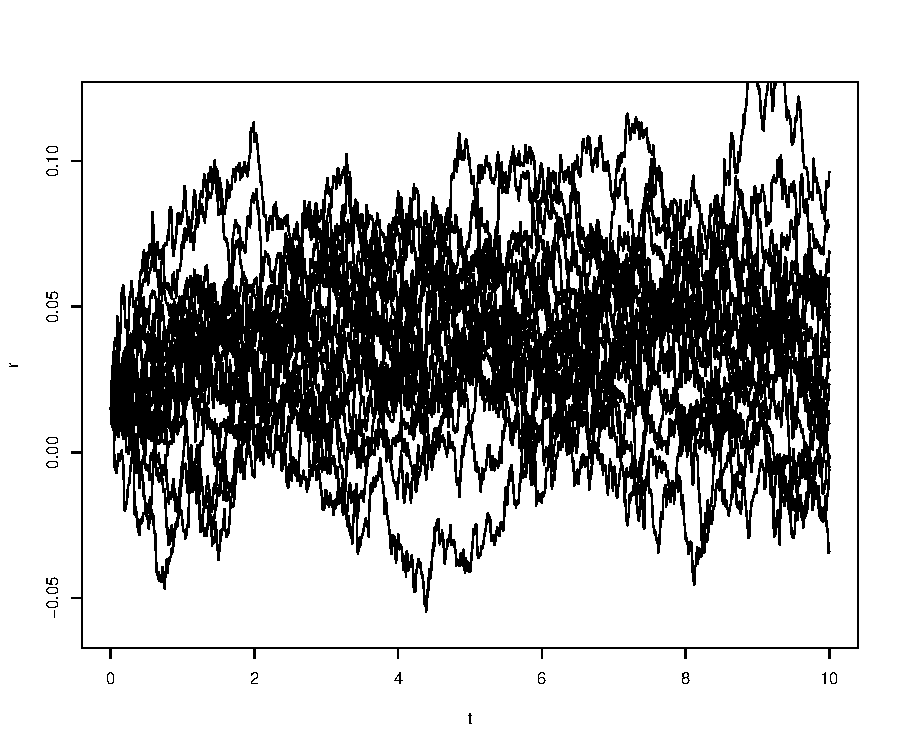
\includegraphics[width=\maxwidth]{figure/p10plot-1} 

\end{knitrout}
		\caption{20 simulated paths of the spot rate under risk neutral measure}
\end{figure}
From the figure above, we observe that the simulated paths follow typical strucure of actual observed spot rate curves. This validates to some extent that our model assumption is valid. 
\subsection{Further Research}
The original plan was actually to work on more advanced Monte Carlo method to estimate zero-coupon bond prices under this model assumption. However, the paper I was reading on this subject was quite intense, and I did not fully understand the methods described in the paper (and marking midterm papers for other courses is taking way longer than I have expected). In the paper, the financial parameters are not assumed to be known in advance, and the only given data in the implementation is the actual observed bond prices with different maturity. The spot rates and the parameters are assumed to follow a complicated joint distribution, so metroplis (or other sampling algorithms) have to be used to obtain the term structure curves. Here is the link to the referenced paper (\url{https://www0.gsb.columbia.edu/mygsb/faculty/research/pubfiles/564/MCMC.pdf})

\end{homeworkProblem}
\end{document}
